%********************************************%
%*       Generated from PreTeXt source      *%
%*       on 2020-07-24T07:50:50-04:00       *%
%*   A recent stable commit (2020-07-07):   *%
%* 1771dacf84bfb1789139598d8379414b560b8f17 *%
%*                                          *%
%*         https://pretextbook.org          *%
%*                                          *%
%********************************************%
\documentclass[oneside,10pt,]{book}
%% Custom Preamble Entries, early (use latex.preamble.early)
%% Default LaTeX packages
%%   1.  always employed (or nearly so) for some purpose, or
%%   2.  a stylewriter may assume their presence
\usepackage{geometry}
%% Some aspects of the preamble are conditional,
%% the LaTeX engine is one such determinant
\usepackage{ifthen}
%% etoolbox has a variety of modern conveniences
\usepackage{etoolbox}
\usepackage{ifxetex,ifluatex}
%% Raster graphics inclusion
\usepackage{graphicx}
%% Color support, xcolor package
%% Always loaded, for: add/delete text, author tools
%% Here, since tcolorbox loads tikz, and tikz loads xcolor
\PassOptionsToPackage{usenames,dvipsnames,svgnames,table}{xcolor}
\usepackage{xcolor}
%% begin: defined colors, via xcolor package, for styling
%% end: defined colors, via xcolor package, for styling
%% Colored boxes, and much more, though mostly styling
%% skins library provides "enhanced" skin, employing tikzpicture
%% boxes may be configured as "breakable" or "unbreakable"
%% "raster" controls grids of boxes, aka side-by-side
\usepackage{tcolorbox}
\tcbuselibrary{skins}
\tcbuselibrary{breakable}
\tcbuselibrary{raster}
%% We load some "stock" tcolorbox styles that we use a lot
%% Placement here is provisional, there will be some color work also
%% First, black on white, no border, transparent, but no assumption about titles
\tcbset{ bwminimalstyle/.style={size=minimal, boxrule=-0.3pt, frame empty,
colback=white, colbacktitle=white, coltitle=black, opacityfill=0.0} }
%% Second, bold title, run-in to text/paragraph/heading
%% Space afterwards will be controlled by environment,
%% independent of constructions of the tcb title
%% Places \blocktitlefont onto many block titles
\tcbset{ runintitlestyle/.style={fonttitle=\blocktitlefont\upshape\bfseries, attach title to upper} }
%% Spacing prior to each exercise, anywhere
\tcbset{ exercisespacingstyle/.style={before skip={1.5ex plus 0.5ex}} }
%% Spacing prior to each block
\tcbset{ blockspacingstyle/.style={before skip={2.0ex plus 0.5ex}} }
%% xparse allows the construction of more robust commands,
%% this is a necessity for isolating styling and behavior
%% The tcolorbox library of the same name loads the base library
\tcbuselibrary{xparse}
%% Hyperref should be here, but likes to be loaded late
%%
%% Inline math delimiters, \(, \), need to be robust
%% 2016-01-31:  latexrelease.sty  supersedes  fixltx2e.sty
%% If  latexrelease.sty  exists, bugfix is in kernel
%% If not, bugfix is in  fixltx2e.sty
%% See:  https://tug.org/TUGboat/tb36-3/tb114ltnews22.pdf
%% and read "Fewer fragile commands" in distribution's  latexchanges.pdf
\IfFileExists{latexrelease.sty}{}{\usepackage{fixltx2e}}
%% Text height identically 9 inches, text width varies on point size
%% See Bringhurst 2.1.1 on measure for recommendations
%% 75 characters per line (count spaces, punctuation) is target
%% which is the upper limit of Bringhurst's recommendations
\geometry{letterpaper,total={340pt,9.0in}}
%% Custom Page Layout Adjustments (use latex.geometry)
%% This LaTeX file may be compiled with pdflatex, xelatex, or lualatex executables
%% LuaTeX is not explicitly supported, but we do accept additions from knowledgeable users
%% The conditional below provides  pdflatex  specific configuration last
%% begin: engine-specific capabilities
\ifthenelse{\boolean{xetex} \or \boolean{luatex}}{%
%% begin: xelatex and lualatex-specific default configuration
\ifxetex\usepackage{xltxtra}\fi
%% realscripts is the only part of xltxtra relevant to lualatex 
\ifluatex\usepackage{realscripts}\fi
%% end:   xelatex and lualatex-specific default configuration
}{
%% begin: pdflatex-specific default configuration
%% We assume a PreTeXt XML source file may have Unicode characters
%% and so we ask LaTeX to parse a UTF-8 encoded file
%% This may work well for accented characters in Western language,
%% but not with Greek, Asian languages, etc.
%% When this is not good enough, switch to the  xelatex  engine
%% where Unicode is better supported (encouraged, even)
\usepackage[utf8]{inputenc}
%% end: pdflatex-specific default configuration
}
%% end:   engine-specific capabilities
%%
%% Fonts.  Conditional on LaTex engine employed.
%% Default Text Font: The Latin Modern fonts are
%% "enhanced versions of the [original TeX] Computer Modern fonts."
%% We use them as the default text font for PreTeXt output.
%% Default Monospace font: Inconsolata (aka zi4)
%% Sponsored by TUG: http://levien.com/type/myfonts/inconsolata.html
%% Loaded for documents with intentional objects requiring monospace
%% See package documentation for excellent instructions
%% fontspec will work universally if we use filename to locate OTF files
%% Loads the "upquote" package as needed, so we don't have to
%% Upright quotes might come from the  textcomp  package, which we also use
%% We employ the shapely \ell to match Google Font version
%% pdflatex: "varl" package option produces shapely \ell
%% pdflatex: "var0" package option produces plain zero (not used)
%% pdflatex: "varqu" package option produces best upright quotes
%% xelatex,lualatex: add OTF StylisticSet 1 for shapely \ell
%% xelatex,lualatex: add OTF StylisticSet 2 for plain zero (not used)
%% xelatex,lualatex: add OTF StylisticSet 3 for upright quotes
%%
%% Automatic Font Control
%% Portions of a document, are, or may, be affected by defined commands
%% These are perhaps more flexible when using  xelatex  rather than  pdflatex
%% The following definitions are meant to be re-defined in a style, using \renewcommand
%% They are scoped when employed (in a TeX group), and so should not be defined with an argument
\newcommand{\divisionfont}{\relax}
\newcommand{\blocktitlefont}{\relax}
\newcommand{\contentsfont}{\relax}
\newcommand{\pagefont}{\relax}
\newcommand{\tabularfont}{\relax}
\newcommand{\xreffont}{\relax}
\newcommand{\titlepagefont}{\relax}
%%
\ifthenelse{\boolean{xetex} \or \boolean{luatex}}{%
%% begin: font setup and configuration for use with xelatex
%% Generally, xelatex is necessary for non-Western fonts
%% fontspec package provides extensive control of system fonts,
%% meaning *.otf (OpenType), and apparently *.ttf (TrueType)
%% that live *outside* your TeX/MF tree, and are controlled by your *system*
%% (it is possible that a TeX distribution will place fonts in a system location)
%%
%% The fontspec package is the best vehicle for using different fonts in  xelatex
%% So we load it always, no matter what a publisher or style might want
%%
\usepackage{fontspec}
%%
%% begin: xelatex main font ("font-xelatex-main" template)
%% Latin Modern Roman is the default font for xelatex and so is loaded with a TU encoding
%% *in the format* so we can't touch it, only perhaps adjust it later
%% in one of two ways (then known by NFSS names such as "lmr")
%% (1) via NFSS with font family names such as "lmr" and "lmss"
%% (2) via fontspec with commands like \setmainfont{Latin Modern Roman}
%% The latter requires the font to be known at the system-level by its font name,
%% but will give access to OTF font features through optional arguments
%% https://tex.stackexchange.com/questions/470008/
%% where-and-how-does-fontspec-sty-specify-the-default-font-latin-modern-roman
%% http://tex.stackexchange.com/questions/115321
%% /how-to-optimize-latin-modern-font-with-xelatex
%%
%% end:   xelatex main font ("font-xelatex-main" template)
%% begin: xelatex mono font ("font-xelatex-mono" template)
%% (conditional on non-trivial uses being present in source)
\IfFontExistsTF{Inconsolatazi4-Regular.otf}{}{\GenericError{}{The font "Inconsolatazi4-Regular.otf" requested by PreTeXt output is not available.  Either a file cannot be located in default locations via a filename, or a font is not known by its name as part of your system.}{Consult the PreTeXt Guide for help with LaTeX fonts.}{}}
\IfFontExistsTF{Inconsolatazi4-Bold.otf}{}{\GenericError{}{The font "Inconsolatazi4-Bold.otf" requested by PreTeXt output is not available.  Either a file cannot be located in default locations via a filename, or a font is not known by its name as part of your system.}{Consult the PreTeXt Guide for help with LaTeX fonts.}{}}
\usepackage{zi4}
\setmonofont[BoldFont=Inconsolatazi4-Bold.otf,StylisticSet={1,3}]{Inconsolatazi4-Regular.otf}
%% end:   xelatex mono font ("font-xelatex-mono" template)
%% begin: xelatex font adjustments ("font-xelatex-style" template)
%% end:   xelatex font adjustments ("font-xelatex-style" template)
%%
%% Extensive support for other languages
\usepackage{polyglossia}
%% Set main/default language based on pretext/@xml:lang value
%% document language code is "en-US", US English
%% usmax variant has extra hypenation
\setmainlanguage[variant=usmax]{english}
%% Enable secondary languages based on discovery of @xml:lang values
%% Enable fonts/scripts based on discovery of @xml:lang values
%% Western languages should be ably covered by Latin Modern Roman
%% end:   font setup and configuration for use with xelatex
}{%
%% begin: font setup and configuration for use with pdflatex
%% begin: pdflatex main font ("font-pdflatex-main" template)
\usepackage{lmodern}
\usepackage[T1]{fontenc}
%% end:   pdflatex main font ("font-pdflatex-main" template)
%% begin: pdflatex mono font ("font-pdflatex-mono" template)
%% (conditional on non-trivial uses being present in source)
\usepackage[varqu,varl]{inconsolata}
%% end:   pdflatex mono font ("font-pdflatex-mono" template)
%% begin: pdflatex font adjustments ("font-pdflatex-style" template)
%% end:   pdflatex font adjustments ("font-pdflatex-style" template)
%% end:   font setup and configuration for use with pdflatex
}
%% Symbols, align environment, commutative diagrams, bracket-matrix
\usepackage{amsmath}
\usepackage{amscd}
\usepackage{amssymb}
%% allow page breaks within display mathematics anywhere
%% level 4 is maximally permissive
%% this is exactly the opposite of AMSmath package philosophy
%% there are per-display, and per-equation options to control this
%% split, aligned, gathered, and alignedat are not affected
\allowdisplaybreaks[4]
%% allow more columns to a matrix
%% can make this even bigger by overriding with  latex.preamble.late  processing option
\setcounter{MaxMatrixCols}{30}
%%
%%
%% Division Titles, and Page Headers/Footers
%% titlesec package, loading "titleps" package cooperatively
%% See code comments about the necessity and purpose of "explicit" option.
%% The "newparttoc" option causes a consistent entry for parts in the ToC 
%% file, but it is only effective if there is a \titleformat for \part.
%% "pagestyles" loads the  titleps  package cooperatively.
\usepackage[explicit, newparttoc, pagestyles]{titlesec}
%% The companion titletoc package for the ToC.
\usepackage{titletoc}
%% Fixes a bug with transition from chapters to appendices in a "book"
%% See generating XSL code for more details about necessity
\newtitlemark{\chaptertitlename}
%% begin: customizations of page styles via the modal "titleps-style" template
%% Designed to use commands from the LaTeX "titleps" package
%% Plain pages should have the same font for page numbers
\renewpagestyle{plain}{%
\setfoot{}{\pagefont\thepage}{}%
}%
%% Single pages as in default LaTeX
\renewpagestyle{headings}{%
\sethead{\pagefont\slshape\MakeUppercase{\ifthechapter{\chaptertitlename\space\thechapter.\space}{}\chaptertitle}}{}{\pagefont\thepage}%
}%
\pagestyle{headings}
%% end: customizations of page styles via the modal "titleps-style" template
%%
%% Create globally-available macros to be provided for style writers
%% These are redefined for each occurence of each division
\newcommand{\divisionnameptx}{\relax}%
\newcommand{\titleptx}{\relax}%
\newcommand{\subtitleptx}{\relax}%
\newcommand{\shortitleptx}{\relax}%
\newcommand{\authorsptx}{\relax}%
\newcommand{\epigraphptx}{\relax}%
%% Create environments for possible occurences of each division
%% Environment for a PTX "preface" at the level of a LaTeX "chapter"
\NewDocumentEnvironment{preface}{mmmmmm}
{%
\renewcommand{\divisionnameptx}{Preface}%
\renewcommand{\titleptx}{#1}%
\renewcommand{\subtitleptx}{#2}%
\renewcommand{\shortitleptx}{#3}%
\renewcommand{\authorsptx}{#4}%
\renewcommand{\epigraphptx}{#5}%
\chapter*{#1}%
\addcontentsline{toc}{chapter}{#3}
\label{#6}%
}{}%
%% Environment for a PTX "chapter" at the level of a LaTeX "chapter"
\NewDocumentEnvironment{chapterptx}{mmmmmm}
{%
\renewcommand{\divisionnameptx}{Chapter}%
\renewcommand{\titleptx}{#1}%
\renewcommand{\subtitleptx}{#2}%
\renewcommand{\shortitleptx}{#3}%
\renewcommand{\authorsptx}{#4}%
\renewcommand{\epigraphptx}{#5}%
\chapter[{#3}]{#1}%
\label{#6}%
}{}%
%% Environment for a PTX "section" at the level of a LaTeX "section"
\NewDocumentEnvironment{sectionptx}{mmmmmm}
{%
\renewcommand{\divisionnameptx}{Section}%
\renewcommand{\titleptx}{#1}%
\renewcommand{\subtitleptx}{#2}%
\renewcommand{\shortitleptx}{#3}%
\renewcommand{\authorsptx}{#4}%
\renewcommand{\epigraphptx}{#5}%
\section[{#3}]{#1}%
\label{#6}%
}{}%
%% Environment for a PTX "subsection" at the level of a LaTeX "subsection"
\NewDocumentEnvironment{subsectionptx}{mmmmmm}
{%
\renewcommand{\divisionnameptx}{Subsection}%
\renewcommand{\titleptx}{#1}%
\renewcommand{\subtitleptx}{#2}%
\renewcommand{\shortitleptx}{#3}%
\renewcommand{\authorsptx}{#4}%
\renewcommand{\epigraphptx}{#5}%
\subsection[{#3}]{#1}%
\label{#6}%
}{}%
%% Environment for a PTX "exercises" at the level of a LaTeX "subsection"
\NewDocumentEnvironment{exercises-subsection}{mmmmmm}
{%
\renewcommand{\divisionnameptx}{Exercises}%
\renewcommand{\titleptx}{#1}%
\renewcommand{\subtitleptx}{#2}%
\renewcommand{\shortitleptx}{#3}%
\renewcommand{\authorsptx}{#4}%
\renewcommand{\epigraphptx}{#5}%
\subsection[{#3}]{#1}%
\label{#6}%
}{}%
%% Environment for a PTX "exercises" at the level of a LaTeX "subsection"
\NewDocumentEnvironment{exercises-subsection-numberless}{mmmmmm}
{%
\renewcommand{\divisionnameptx}{Exercises}%
\renewcommand{\titleptx}{#1}%
\renewcommand{\subtitleptx}{#2}%
\renewcommand{\shortitleptx}{#3}%
\renewcommand{\authorsptx}{#4}%
\renewcommand{\epigraphptx}{#5}%
\subsection*{#1}%
\addcontentsline{toc}{subsection}{#3}
\label{#6}%
}{}%
%% Environment for a PTX "appendix" at the level of a LaTeX "chapter"
\NewDocumentEnvironment{appendixptx}{mmmmmm}
{%
\renewcommand{\divisionnameptx}{Appendix}%
\renewcommand{\titleptx}{#1}%
\renewcommand{\subtitleptx}{#2}%
\renewcommand{\shortitleptx}{#3}%
\renewcommand{\authorsptx}{#4}%
\renewcommand{\epigraphptx}{#5}%
\chapter[{#3}]{#1}%
\label{#6}%
}{}%
%% Environment for a PTX "references" at the level of a LaTeX "chapter"
\NewDocumentEnvironment{references-chapter}{mmmmmm}
{%
\renewcommand{\divisionnameptx}{References}%
\renewcommand{\titleptx}{#1}%
\renewcommand{\subtitleptx}{#2}%
\renewcommand{\shortitleptx}{#3}%
\renewcommand{\authorsptx}{#4}%
\renewcommand{\epigraphptx}{#5}%
\chapter[{#3}]{#1}%
\label{#6}%
}{}%
%% Environment for a PTX "references" at the level of a LaTeX "chapter"
\NewDocumentEnvironment{references-chapter-numberless}{mmmmmm}
{%
\renewcommand{\divisionnameptx}{References}%
\renewcommand{\titleptx}{#1}%
\renewcommand{\subtitleptx}{#2}%
\renewcommand{\shortitleptx}{#3}%
\renewcommand{\authorsptx}{#4}%
\renewcommand{\epigraphptx}{#5}%
\chapter*{#1}%
\addcontentsline{toc}{chapter}{#3}
\label{#6}%
}{}%
%% Environment for a PTX "index" at the level of a LaTeX "chapter"
\NewDocumentEnvironment{indexptx}{mmmmmm}
{%
\renewcommand{\divisionnameptx}{Index}%
\renewcommand{\titleptx}{#1}%
\renewcommand{\subtitleptx}{#2}%
\renewcommand{\shortitleptx}{#3}%
\renewcommand{\authorsptx}{#4}%
\renewcommand{\epigraphptx}{#5}%
\chapter*{#1}%
\addcontentsline{toc}{chapter}{#3}
\label{#6}%
}{}%
%%
%% Styles for six traditional LaTeX divisions
\titleformat{\part}[display]
{\divisionfont\Huge\bfseries\centering}{\divisionnameptx\space\thepart}{30pt}{\Huge#1}
[{\Large\centering\authorsptx}]
\titleformat{\chapter}[display]
{\divisionfont\huge\bfseries}{\divisionnameptx\space\thechapter}{20pt}{\Huge#1}
[{\Large\authorsptx}]
\titleformat{name=\chapter,numberless}[display]
{\divisionfont\huge\bfseries}{}{0pt}{#1}
[{\Large\authorsptx}]
\titlespacing*{\chapter}{0pt}{50pt}{40pt}
\titleformat{\section}[hang]
{\divisionfont\Large\bfseries}{\thesection}{1ex}{#1}
[{\large\authorsptx}]
\titleformat{name=\section,numberless}[block]
{\divisionfont\Large\bfseries}{}{0pt}{#1}
[{\large\authorsptx}]
\titlespacing*{\section}{0pt}{3.5ex plus 1ex minus .2ex}{2.3ex plus .2ex}
\titleformat{\subsection}[hang]
{\divisionfont\large\bfseries}{\thesubsection}{1ex}{#1}
[{\normalsize\authorsptx}]
\titleformat{name=\subsection,numberless}[block]
{\divisionfont\large\bfseries}{}{0pt}{#1}
[{\normalsize\authorsptx}]
\titlespacing*{\subsection}{0pt}{3.25ex plus 1ex minus .2ex}{1.5ex plus .2ex}
\titleformat{\subsubsection}[hang]
{\divisionfont\normalsize\bfseries}{\thesubsubsection}{1em}{#1}
[{\small\authorsptx}]
\titleformat{name=\subsubsection,numberless}[block]
{\divisionfont\normalsize\bfseries}{}{0pt}{#1}
[{\normalsize\authorsptx}]
\titlespacing*{\subsubsection}{0pt}{3.25ex plus 1ex minus .2ex}{1.5ex plus .2ex}
\titleformat{\paragraph}[hang]
{\divisionfont\normalsize\bfseries}{\theparagraph}{1em}{#1}
[{\small\authorsptx}]
\titleformat{name=\paragraph,numberless}[block]
{\divisionfont\normalsize\bfseries}{}{0pt}{#1}
[{\normalsize\authorsptx}]
\titlespacing*{\paragraph}{0pt}{3.25ex plus 1ex minus .2ex}{1.5em}
%%
%% Styles for five traditional LaTeX divisions
\titlecontents{part}%
[0pt]{\contentsmargin{0em}\addvspace{1pc}\contentsfont\bfseries}%
{\Large\thecontentslabel\enspace}{\Large}%
{}%
[\addvspace{.5pc}]%
\titlecontents{chapter}%
[0pt]{\contentsmargin{0em}\addvspace{1pc}\contentsfont\bfseries}%
{\large\thecontentslabel\enspace}{\large}%
{\hfill\bfseries\thecontentspage}%
[\addvspace{.5pc}]%
\dottedcontents{section}[3.8em]{\contentsfont}{2.3em}{1pc}%
\dottedcontents{subsection}[6.1em]{\contentsfont}{3.2em}{1pc}%
\dottedcontents{subsubsection}[9.3em]{\contentsfont}{4.3em}{1pc}%
%%
%% Begin: Semantic Macros
%% To preserve meaning in a LaTeX file
%%
%% \mono macro for content of "c", "cd", "tag", etc elements
%% Also used automatically in other constructions
%% Simply an alias for \texttt
%% Always defined, even if there is no need, or if a specific tt font is not loaded
\newcommand{\mono}[1]{\texttt{#1}}
%%
%% Following semantic macros are only defined here if their
%% use is required only in this specific document
%%
%% Used for inline definitions of terms
\newcommand{\terminology}[1]{\textbf{#1}}
%% End: Semantic Macros
%% Division Numbering: Chapters, Sections, Subsections, etc
%% Division numbers may be turned off at some level ("depth")
%% A section *always* has depth 1, contrary to us counting from the document root
%% The latex default is 3.  If a larger number is present here, then
%% removing this command may make some cross-references ambiguous
%% The precursor variable $numbering-maxlevel is checked for consistency in the common XSL file
\setcounter{secnumdepth}{3}
%%
%% AMS "proof" environment is no longer used, but we leave previously
%% implemented \qedhere in place, should the LaTeX be recycled
\newcommand{\qedhere}{\relax}
%%
%% A faux tcolorbox whose only purpose is to provide common numbering
%% facilities for most blocks (possibly not projects, 2D displays)
%% Controlled by  numbering.theorems.level  processing parameter
\newtcolorbox[auto counter, number within=section]{block}{}
%%
%% This document is set to number PROJECT-LIKE on a separate numbering scheme
%% So, a faux tcolorbox whose only purpose is to provide this numbering
%% Controlled by  numbering.projects.level  processing parameter
\newtcolorbox[auto counter, number within=section]{project-distinct}{}
%% A faux tcolorbox whose only purpose is to provide common numbering
%% facilities for 2D displays which are subnumbered as part of a "sidebyside"
\newtcolorbox[auto counter, number within=tcb@cnt@block, number freestyle={\noexpand\thetcb@cnt@block(\noexpand\alph{\tcbcounter})}]{subdisplay}{}
%%
%% tcolorbox, with styles, for THEOREM-LIKE
%%
%% theorem: fairly simple numbered block/structure
\tcbset{ theoremstyle/.style={bwminimalstyle, runintitlestyle, blockspacingstyle, after title={\space}, } }
\newtcolorbox[use counter from=block]{theorem}[3]{title={{Theorem~\thetcbcounter\notblank{#1#2}{\space}{}\notblank{#1}{\space#1}{}\notblank{#2}{\space(#2)}{}}}, phantomlabel={#3}, breakable, parbox=false, after={\par}, fontupper=\itshape, theoremstyle, }
%% corollary: fairly simple numbered block/structure
\tcbset{ corollarystyle/.style={bwminimalstyle, runintitlestyle, blockspacingstyle, after title={\space}, } }
\newtcolorbox[use counter from=block]{corollary}[3]{title={{Corollary~\thetcbcounter\notblank{#1#2}{\space}{}\notblank{#1}{\space#1}{}\notblank{#2}{\space(#2)}{}}}, phantomlabel={#3}, breakable, parbox=false, after={\par}, fontupper=\itshape, corollarystyle, }
%%
%% tcolorbox, with styles, for DEFINITION-LIKE
%%
%% definition: fairly simple numbered block/structure
\tcbset{ definitionstyle/.style={bwminimalstyle, runintitlestyle, blockspacingstyle, after title={\space}, after upper={\space\space\hspace*{\stretch{1}}\(\lozenge\)}, } }
\newtcolorbox[use counter from=block]{definition}[2]{title={{Definition~\thetcbcounter\notblank{#1}{\space\space#1}{}}}, phantomlabel={#2}, breakable, parbox=false, after={\par}, definitionstyle, }
%%
%% tcolorbox, with styles, for EXAMPLE-LIKE
%%
%% example: fairly simple numbered block/structure
\tcbset{ examplestyle/.style={bwminimalstyle, runintitlestyle, blockspacingstyle, after title={\space}, after upper={\space\space\hspace*{\stretch{1}}\(\square\)}, } }
\newtcolorbox[use counter from=block]{example}[2]{title={{Example~\thetcbcounter\notblank{#1}{\space\space#1}{}}}, phantomlabel={#2}, breakable, parbox=false, after={\par}, examplestyle, }
%%
%% tcolorbox, with styles, for FIGURE-LIKE
%%
%% figureptx: 2-D display structure
\tcbset{ figureptxstyle/.style={bwminimalstyle, middle=1ex, blockspacingstyle, fontlower=\blocktitlefont} }
\newtcolorbox[use counter from=block]{figureptx}[3]{lower separated=false, before lower={{\textbf{Figure~\thetcbcounter}\space#1}}, phantomlabel={#2}, unbreakable, parbox=false, figureptxstyle, }
%% tableptx: 2-D display structure
\tcbset{ tableptxstyle/.style={bwminimalstyle, middle=1ex, blockspacingstyle, coltitle=black, bottomtitle=2ex, titlerule=-0.3pt, fonttitle=\blocktitlefont} }
\newtcolorbox[use counter from=block]{tableptx}[3]{title={{\textbf{Table~\thetcbcounter}\space#1}}, phantomlabel={#2}, unbreakable, parbox=false, tableptxstyle, }
%%
%% xparse environments for introductions and conclusions of divisions
%%
%% introduction: in a structured division
\NewDocumentEnvironment{introduction}{m}
{\notblank{#1}{\noindent\textbf{#1}\space}{}}{\par\medskip}
%%
%% tcolorbox, with styles, for miscellaneous environments
%%
%% proof: title is a replacement
\tcbset{ proofstyle/.style={bwminimalstyle, fonttitle=\blocktitlefont\itshape, attach title to upper, after title={\space}, after upper={\space\space\hspace*{\stretch{1}}\(\blacksquare\)},
} }
\newtcolorbox{proof}[2]{title={\notblank{#1}{#1}{Proof.}}, phantom={\hypertarget{#2}{}}, breakable, parbox=false, after={\par}, proofstyle }
%% Divisional exercises (and worksheet) as LaTeX environments
%% Third argument is option for extra workspace in worksheets
%% Hanging indent occupies a 5ex width slot prior to left margin
%% Experimentally this seems just barely sufficient for a bold "888."
%% Division exercises, not in exercise group
\tcbset{ divisionexercisestyle/.style={bwminimalstyle, runintitlestyle, exercisespacingstyle, left=5ex, breakable, parbox=false } }
\newtcolorbox{divisionexercise}[4]{divisionexercisestyle, before title={\hspace{-5ex}\makebox[5ex][l]{#1.}}, title={\notblank{#2}{#2\space}{}}, phantom={\hypertarget{#4}{}}, after={\notblank{#3}{\newline\rule{\workspacestrutwidth}{#3\textheight}\newline}{}}}
%% Localize LaTeX supplied names (possibly none)
\renewcommand*{\appendixname}{Appendix}
\renewcommand*{\chaptername}{Chapter}
%% "tcolorbox" environment for a single image, occupying entire \linewidth
%% arguments are left-margin, width, right-margin, as multiples of
%% \linewidth, and are guaranteed to be positive and sum to 1.0
\tcbset{ imagestyle/.style={bwminimalstyle} }
\NewTColorBox{image}{mmm}{imagestyle,left skip=#1\linewidth,width=#2\linewidth}
%% For improved tables
\usepackage{array}
%% Some extra height on each row is desirable, especially with horizontal rules
%% Increment determined experimentally
\setlength{\extrarowheight}{0.2ex}
%% Define variable thickness horizontal rules, full and partial
%% Thicknesses are 0.03, 0.05, 0.08 in the  booktabs  package
\newcommand{\hrulethin}  {\noalign{\hrule height 0.04em}}
\newcommand{\hrulemedium}{\noalign{\hrule height 0.07em}}
\newcommand{\hrulethick} {\noalign{\hrule height 0.11em}}
%% We preserve a copy of the \setlength package before other
%% packages (extpfeil) get a chance to load packages that redefine it
\let\oldsetlength\setlength
\newlength{\Oldarrayrulewidth}
\newcommand{\crulethin}[1]%
{\noalign{\global\oldsetlength{\Oldarrayrulewidth}{\arrayrulewidth}}%
\noalign{\global\oldsetlength{\arrayrulewidth}{0.04em}}\cline{#1}%
\noalign{\global\oldsetlength{\arrayrulewidth}{\Oldarrayrulewidth}}}%
\newcommand{\crulemedium}[1]%
{\noalign{\global\oldsetlength{\Oldarrayrulewidth}{\arrayrulewidth}}%
\noalign{\global\oldsetlength{\arrayrulewidth}{0.07em}}\cline{#1}%
\noalign{\global\oldsetlength{\arrayrulewidth}{\Oldarrayrulewidth}}}
\newcommand{\crulethick}[1]%
{\noalign{\global\oldsetlength{\Oldarrayrulewidth}{\arrayrulewidth}}%
\noalign{\global\oldsetlength{\arrayrulewidth}{0.11em}}\cline{#1}%
\noalign{\global\oldsetlength{\arrayrulewidth}{\Oldarrayrulewidth}}}
%% Single letter column specifiers defined via array package
\newcolumntype{A}{!{\vrule width 0.04em}}
\newcolumntype{B}{!{\vrule width 0.07em}}
\newcolumntype{C}{!{\vrule width 0.11em}}
%% Program listing support: for listings, programs, consoles, and Sage code
\ifthenelse{\boolean{xetex} \or \boolean{luatex}}%
  {\tcbuselibrary{listings}}%
  {\tcbuselibrary{listingsutf8}}%
%% We define the listings font style to be the default "ttfamily"
%% To fix hyphens/dashes rendered in PDF as fancy minus signs by listing
%% http://tex.stackexchange.com/questions/33185/listings-package-changes-hyphens-to-minus-signs
\makeatletter
\lst@CCPutMacro\lst@ProcessOther {"2D}{\lst@ttfamily{-{}}{-{}}}
\@empty\z@\@empty
\makeatother
%% We define a null language, free of any formatting or style
%% for use when a language is not supported, or pseudo-code, or consoles
%% Not necessary for Sage code, so in limited cases included unnecessarily
\lstdefinelanguage{none}{identifierstyle=,commentstyle=,stringstyle=,keywordstyle=}
\ifthenelse{\boolean{xetex}}{}{%
%% begin: pdflatex-specific listings configuration
%% translate U+0080 - U+00F0 to their textmode LaTeX equivalents
%% Data originally from https://www.w3.org/Math/characters/unicode.xml, 2016-07-23
%% Lines marked in XSL with "$" were converted from mathmode to textmode
\lstset{extendedchars=true}
\lstset{literate={ }{{~}}{1}{¡}{{\textexclamdown }}{1}{¢}{{\textcent }}{1}{£}{{\textsterling }}{1}{¤}{{\textcurrency }}{1}{¥}{{\textyen }}{1}{¦}{{\textbrokenbar }}{1}{§}{{\textsection }}{1}{¨}{{\textasciidieresis }}{1}{©}{{\textcopyright }}{1}{ª}{{\textordfeminine }}{1}{«}{{\guillemotleft }}{1}{¬}{{\textlnot }}{1}{­}{{\-}}{1}{®}{{\textregistered }}{1}{¯}{{\textasciimacron }}{1}{°}{{\textdegree }}{1}{±}{{\textpm }}{1}{²}{{\texttwosuperior }}{1}{³}{{\textthreesuperior }}{1}{´}{{\textasciiacute }}{1}{µ}{{\textmu }}{1}{¶}{{\textparagraph }}{1}{·}{{\textperiodcentered }}{1}{¸}{{\c{}}}{1}{¹}{{\textonesuperior }}{1}{º}{{\textordmasculine }}{1}{»}{{\guillemotright }}{1}{¼}{{\textonequarter }}{1}{½}{{\textonehalf }}{1}{¾}{{\textthreequarters }}{1}{¿}{{\textquestiondown }}{1}{À}{{\`{A}}}{1}{Á}{{\'{A}}}{1}{Â}{{\^{A}}}{1}{Ã}{{\~{A}}}{1}{Ä}{{\"{A}}}{1}{Å}{{\AA }}{1}{Æ}{{\AE }}{1}{Ç}{{\c{C}}}{1}{È}{{\`{E}}}{1}{É}{{\'{E}}}{1}{Ê}{{\^{E}}}{1}{Ë}{{\"{E}}}{1}{Ì}{{\`{I}}}{1}{Í}{{\'{I}}}{1}{Î}{{\^{I}}}{1}{Ï}{{\"{I}}}{1}{Ð}{{\DH }}{1}{Ñ}{{\~{N}}}{1}{Ò}{{\`{O}}}{1}{Ó}{{\'{O}}}{1}{Ô}{{\^{O}}}{1}{Õ}{{\~{O}}}{1}{Ö}{{\"{O}}}{1}{×}{{\texttimes }}{1}{Ø}{{\O }}{1}{Ù}{{\`{U}}}{1}{Ú}{{\'{U}}}{1}{Û}{{\^{U}}}{1}{Ü}{{\"{U}}}{1}{Ý}{{\'{Y}}}{1}{Þ}{{\TH }}{1}{ß}{{\ss }}{1}{à}{{\`{a}}}{1}{á}{{\'{a}}}{1}{â}{{\^{a}}}{1}{ã}{{\~{a}}}{1}{ä}{{\"{a}}}{1}{å}{{\aa }}{1}{æ}{{\ae }}{1}{ç}{{\c{c}}}{1}{è}{{\`{e}}}{1}{é}{{\'{e}}}{1}{ê}{{\^{e}}}{1}{ë}{{\"{e}}}{1}{ì}{{\`{\i}}}{1}{í}{{\'{\i}}}{1}{î}{{\^{\i}}}{1}{ï}{{\"{\i}}}{1}{ð}{{\dh }}{1}{ñ}{{\~{n}}}{1}{ò}{{\`{o}}}{1}{ó}{{\'{o}}}{1}{ô}{{\^{o}}}{1}{õ}{{\~{o}}}{1}{ö}{{\"{o}}}{1}{÷}{{\textdiv }}{1}{ø}{{\o }}{1}{ù}{{\`{u}}}{1}{ú}{{\'{u}}}{1}{û}{{\^{u}}}{1}{ü}{{\"{u}}}{1}{ý}{{\'{y}}}{1}{þ}{{\th }}{1}{ÿ}{{\"{y}}}{1}}
%% end: pdflatex-specific listings configuration
}
%% End of generic listing adjustments
%% The listings package as tcolorbox for Sage code
%% We do as much styling as possible with tcolorbox, not listings
%% Sage's blue is 50%, we go way lighter (blue!05 would also work)
%% Note that we defuse listings' default "aboveskip" and "belowskip"
\definecolor{sageblue}{rgb}{0.95,0.95,1}
\tcbset{ sagestyle/.style={left=0pt, right=0pt, top=0ex, bottom=0ex, middle=0pt, toptitle=0pt, bottomtitle=0pt,
boxsep=4pt, listing only, fontupper=\small\ttfamily,
breakable, parbox=false, 
listing options={language=Python,breaklines=true,breakatwhitespace=true, extendedchars=true, aboveskip=0pt, belowskip=0pt}} }
\newtcblisting{sageinput}{sagestyle, colback=sageblue, sharp corners, boxrule=0.5pt, toprule at break=-0.3pt, bottomrule at break=-0.3pt, }
\newtcblisting{sageoutput}{sagestyle, colback=white, colframe=white, frame empty, before skip=0pt, after skip=0pt, }
%% Multiple column, column-major lists
\usepackage{multicol}
%% More flexible list management, esp. for references
%% But also for specifying labels (i.e. custom order) on nested lists
\usepackage{enumitem}
%% Lists of references in their own section, maximum depth 1
\newlist{referencelist}{description}{4}
\setlist[referencelist]{leftmargin=!,labelwidth=!,labelsep=0ex,itemsep=1.0ex,topsep=1.0ex,partopsep=0pt,parsep=0pt}
%% Support for index creation
%% imakeidx package does not require extra pass (as with makeidx)
%% Title of the "Index" section set via a keyword
%% Language support for the "see" and "see also" phrases
\usepackage{imakeidx}
\makeindex[title=Index, intoc=true]
\renewcommand{\seename}{See}
\renewcommand{\alsoname}{See also}
%% Package for tables spanning several pages
\usepackage{longtable}
%% hyperref driver does not need to be specified, it will be detected
%% Footnote marks in tcolorbox have broken linking under
%% hyperref, so it is necessary to turn off all linking
%% It *must* be given as a package option, not with \hypersetup
\usepackage[hyperfootnotes=false]{hyperref}
%% configure hyperref's  \url  to match listings' inline verbatim
\renewcommand\UrlFont{\small\ttfamily}
%% Hyperlinking active in electronic PDFs, all links solid and blue
\hypersetup{colorlinks=true,linkcolor=blue,citecolor=blue,filecolor=blue,urlcolor=blue}
\hypersetup{pdftitle={Applied Discrete Structures}}
%% If you manually remove hyperref, leave in this next command
\providecommand\phantomsection{}
%% Graphics Preamble Entries
\usepackage{amsmath}
%% If tikz has been loaded, replace ampersand with \amp macro
%% extpfeil package for certain extensible arrows,
%% as also provided by MathJax extension of the same name
%% NB: this package loads mtools, which loads calc, which redefines
%%     \setlength, so it can be removed if it seems to be in the 
%%     way and your math does not use:
%%     
%%     \xtwoheadrightarrow, \xtwoheadleftarrow, \xmapsto, \xlongequal, \xtofrom
%%     
%%     we have had to be extra careful with variable thickness
%%     lines in tables, and so also load this package late
\usepackage{extpfeil}
%% Custom Preamble Entries, late (use latex.preamble.late)
%% Begin: Author-provided packages
%% (From  docinfo/latex-preamble/package  elements)
%% End: Author-provided packages
%% Begin: Author-provided macros
%% (From  docinfo/macros  element)
%% Plus three from MBX for XML characters
\newcommand{\identity}{\mathrm{id}}
\newcommand{\notdivide}{{\not{\mid}}}
\newcommand{\notsubset}{\not\subset}
\newcommand{\lcm}{\operatorname{lcm}}
\newcommand{\gf}{\operatorname{GF}}
\newcommand{\inn}{\operatorname{Inn}}
\newcommand{\aut}{\operatorname{Aut}}
\newcommand{\Hom}{\operatorname{Hom}}
\newcommand{\cis}{\operatorname{cis}}
\newcommand{\chr}{\operatorname{char}}
\newcommand{\Null}{\operatorname{Null}}
\renewcommand{\vec}[1]{\mathbf{#1}}
\newcommand{\lt}{<}
\newcommand{\gt}{>}
\newcommand{\amp}{&}
%% End: Author-provided macros
\begin{document}
\frontmatter
%% begin: half-title
\thispagestyle{empty}
{\titlepagefont\centering
\vspace*{0.28\textheight}
{\Huge Applied Discrete Structures}\\}
\clearpage
%% end:   half-title
%% begin: adcard
\thispagestyle{empty}
\null%
\clearpage
%% end:   adcard
%% begin: title page
%% Inspired by Peter Wilson's "titleDB" in "titlepages" CTAN package
\thispagestyle{empty}
{\titlepagefont\centering
\vspace*{0.14\textheight}
%% Target for xref to top-level element is ToC
\addtocontents{toc}{\protect\hypertarget{x:book:ic}{}}
{\Huge Applied Discrete Structures}\\[3\baselineskip]
{\Large Al Doerr}\\[0.5\baselineskip]
{\Large University of Massachusetts Lowell}\\[3\baselineskip]
{\Large Ken Levasseur}\\[0.5\baselineskip]
{\Large University of Massachusetts Lowell}\\[3\baselineskip]
{\Large 2016}\\}
\clearpage
%% end:   title page
%% begin: copyright-page
\thispagestyle{empty}
\hypertarget{g:colophon:idm352001309120}{}\vspace*{\stretch{2}}
\noindent{\bfseries Edition}: 3rd Edition\par\medskip
\noindent{\bfseries Website}: \href{http:\slash{}\slash{}faculty.uml.edu\slash{}klevasseur\slash{}ADS2}{faculty.uml.edu\slash{}klevasseur\slash{}ADS2}\par\medskip
\noindent\textcopyright{}2016\quad{}Al Doerr, Ken Levasseur\\[0.5\baselineskip]
Applied Discrete Structures by Alan Doerr and Kenneth Levasseur is licensed under a Creative Commons Attribution-NonCommercial-ShareAlike 3.0 United States License. You are free to Share: copy and redistribute the material in any medium or format; Adapt: remix, transform, and build upon the material. You may not use the material for commercial purposes.  The licensor cannot revoke these freedoms as long as you follow the license terms.\par\medskip
\vspace*{\stretch{1}}
\null\clearpage
%% end:   copyright-page
%
%
\typeout{************************************************}
\typeout{Preface  Preface}
\typeout{************************************************}
%
\begin{preface}{Preface}{}{Preface}{}{}{x:preface:ads-preface}
\emph{Applied Discrete Structures} is designed for use in a university course in discrete mathematics spanning up two semesters.   Its original design was for computer science majors to be introduced to the mathematical topics that are useful in computer science.   It can also serve the same purpose for mathematics majors, providing a first exposure to many essential topics.%
\par
We embarked on this open-source project in 2010, twenty-one years after the publication of the 2nd edition of \emph{Applied Discrete Structures for Computer Science} inn 1989.  Since then, the publishing and computing landscapes have both changed dramatically. We signed a contract for the second edition with Science Research Associates in 1988 but by the time the book was ready to print, SRA had been sold to MacMillan. Soon after, the rights had been passed on to Pearson Education, Inc. In 2010, the long-term future of printed textbooks is uncertain. In the meantime, textbook prices (both printed and e-books) have increased and a growing open source textbook market movement has started. One of our objectives in revisiting this text is to make it available to our students in an affordable format. In its original form, the text was peer-reviewed and was adopted for use at several universities throughout the country. For this reason, we see \emph{Applied Discrete Structures} as not only an inexpensive alternative, but a high quality alternative.%
\par
An initial choice of Mathematica for ``source code'' was based on the speed with which we could do the conversion.  However, the format was not ideal, with no viable web version available.  The project has been well-received in spite of these issues.  Validation through the listing of this project on the American Institute of Mathematics was very helpful. This version of \emph{Applied Discrete Structures} has been developed using \emph{PreTeXt}, a lightweight XML application for authors of scientific articles, textbooks and monographs initiated by Rob Beezer, U. of Puget Sound.  When the PreTeXt project was launched, it was the natural next step.  The features of PreTeXt make it far more readable, with easy production of web, pdf and print formats.%
\par
As indicated above, the computing landscape is very different from the 1980's and this accounts for the most significant changes in the text. One of the most common programming languages of the 1980's was Pascal.  We used it to illustrate many of the concepts in the text.  Although it isn't totally dead, Pascal is far from the mainstream of computing in the 21st century.  The open source software movement was just starting in the late 1980's and in 2005, the first version of Sage (later renamed SageMath), an open-source computer algebra system, was first released. In Applied Discrete Structures we have replaced "Pascal Notes" with "SageMath Notes."%
\par
Many of the concepts introduced in this text are illustrated using SageMath code.  SageMath (\href{http://sagemath.org}{sagemath.org}) is a free, open source, software system for advanced mathematics.  Sage can be used either on your own computer, a local server, or on SageMathCloud (\href{https://cloud.sagemath.com}{https:\slash{}\slash{}cloud.sagemath.com}).%
\nopagebreak\par%
\hfill\begin{tabular}[t]{l@{}}
Ken Levasseur\\
Lowell, MA
\end{tabular}\\\par
\end{preface}
%% begin: table of contents
%% Adjust Table of Contents
\setcounter{tocdepth}{1}
\renewcommand*\contentsname{Contents}
\tableofcontents
%% end:   table of contents
\mainmatter
%
%
\typeout{************************************************}
\typeout{Chapter 1 More on Sets}
\typeout{************************************************}
%
\begin{chapterptx}{More on Sets}{}{More on Sets}{}{}{x:chapter:chapter_4}
\begin{introduction}{}%
In this chapter we shall look more closely at some basic facts about sets. One question we could ask ourselves is: Can we manipulate sets similarly to the way we manipulated expressions in basic algebra, or to the way we manipulated propositions in logic? In basic algebra we are aware that \(a \cdot  (b + c) = a\cdot  b + a \cdot  c\) for all real numbers \(a\), \(b\), and \(c\). In logic we verified an analogue of this statement, namely, \(p
\land  ( q \lor  r) \Leftrightarrow  (p \land  q)\lor  (p \land  r))\), where \(p, q, \textrm{ and } r\) were arbitrary propositions. If \(A\), \(B\), and \(C\) are arbitrary sets, is \(A \cap  (B \cup  C) = (A \cap  B) \cup  (A \cap  C)\)? How do we convince ourselves of it is truth, or discover that it is false? Let us consider some approaches to this problem, look at their pros and cons, and determine their validity.  Later in this chapter, we introduce partitions of sets and minsets.%
\end{introduction}%
%
%
\typeout{************************************************}
\typeout{Section 1.1 Methods of Proof for Sets}
\typeout{************************************************}
%
\begin{sectionptx}{Methods of Proof for Sets}{}{Methods of Proof for Sets}{}{}{x:section:s-proof-methods-sets}
\begin{introduction}{}%
If \(A\), \(B\), and \(C\) are arbitrary sets, is it always true that \(A \cap  (B \cup  C) = (A \cap  B) \cup  (A \cap  C)\)?  There are a variety of ways that we could attempt to prove that this distributive law for intersection over union is indeed true.  We start with a common ``non-proof'' and then work toward more acceptable methods.%
\end{introduction}%
%
%
\typeout{************************************************}
\typeout{Subsection 1.1.1 Examples and Counterexamples}
\typeout{************************************************}
%
\begin{subsectionptx}{Examples and Counterexamples}{}{Examples and Counterexamples}{}{}{x:subsection:ss-examples-and-counterexamples}
We could, for example, let \(A = \{1, 2\}\), \(B = \{5, 8, 10\}\), and \(C = \{3, 2, 5\}\), and determine whether the distributive law is true for these values of \(A\), \(B\), and \(C\). In doing this we will have only determined that the distributive law is true for this one example. It does not prove the distributive law for all possible sets \(A\), \(B\), and \(C\) and hence is an invalid method of proof. However, trying a few examples has considerable merit insofar as it makes us more comfortable with the statement in question. Indeed, if the statement is not true for the example, we have disproved the statement.%
\begin{definition}{Counterexample.}{x:definition:def-counterexample}%
An example that disproves a statement is called a counterexample.%
\end{definition}
\begin{example}{Disproving distributivity of addition over multiplication.}{x:example:ex-addition-over-mult}%
From basic algebra we learned that multiplication is distributive over addition. Is addition distributive over multiplication? That is, is \(a + (b \cdot  c) = (a + b) \cdot  (a + c)\) always true? If we choose the values \(a = 3\), \(b = 4\), and \(c = 1\), we find that \(3 + (4 \cdot  1) \neq  (3 + 4)\cdot (3 + 1)\). Therefore, this set of values serves as a counterexample to a distributive law of addition over multiplication.%
\end{example}
\end{subsectionptx}
%
%
\typeout{************************************************}
\typeout{Subsection 1.1.2 Proof Using Venn Diagrams}
\typeout{************************************************}
%
\begin{subsectionptx}{Proof Using Venn Diagrams}{}{Proof Using Venn Diagrams}{}{}{x:subsection:ss-venn-proofs}
In this method, we illustrate both sides of the statement via a Venn diagram and determine whether both Venn diagrams give us the same ``picture,'' For example, the left side of the distributive law is developed in \hyperref[x:figure:distrib-venn-lhs]{Figure~{\xreffont\ref{x:figure:distrib-venn-lhs}}} and the right side in \hyperref[x:figure:distrib-venn-rhs]{Figure~{\xreffont\ref{x:figure:distrib-venn-rhs}}}. Note that the final results give you the same shaded area.%
\par
The advantage of this method is that it is relatively quick and mechanical. The disadvantage is that it is workable only if there are a small number of sets under consideration. In addition, it doesn't work very well in a static environment like a book or test paper.  Venn diagrams tend to work well if you have a potentially dynamic environment like a blackboard or video.%
\begin{figureptx}{Development of the left side of the distributive law for sets}{x:figure:distrib-venn-lhs}{}%
\begin{image}{0}{1}{0}%
\includegraphics[width=\linewidth]{images/distrib-venn-lhs.png}
\end{image}%
\tcblower
\end{figureptx}%
\begin{figureptx}{Development of the right side of the distributive law for sets}{x:figure:distrib-venn-rhs}{}%
\begin{image}{0}{1}{0}%
\includegraphics[width=\linewidth]{images/distrib-venn-rhs.png}
\end{image}%
\tcblower
\end{figureptx}%
\end{subsectionptx}
%
%
\typeout{************************************************}
\typeout{Subsection 1.1.3 Proof using Set-membership Tables}
\typeout{************************************************}
%
\begin{subsectionptx}{Proof using Set-membership Tables}{}{Proof using Set-membership Tables}{}{}{x:subsection:ss-membership-table-proof}
Let \(A\) be a subset of a universal set \(U\) and let \(u\in U\). To use this method we note that exactly one of the following is true: \(u \in  A\) or \(u\notin  A\). Denote the situation where \(u \in  A\) by 1 and that where \(u \notin  A\) by 0. Working with two sets, \(A\) and \(B\), and if \(u \in  U\), there are four possible outcomes of ``where \(u\) can be.'' What are they? The set-membership table for \(A \cup  B\) is:%
\begin{tableptx}{\textbf{Membership Table for \(A \cup  B\)}}{x:table:mt-union}{}%
\centering
{\tabularfont%
\begin{tabular}{ccc}
\(A\)&\(B\)&\(A \cup  B\)\tabularnewline[0pt]
0&0&0\tabularnewline[0pt]
0&1&1\tabularnewline[0pt]
1&0&1\tabularnewline[0pt]
1&1&1
\end{tabular}
}%
\end{tableptx}%
This table illustrates that \(u\in A \cup  B\) if and only if \(u\in A\) or \(u \in  B\).%
\par
In order to prove the distributive law via a set-membership table, write out the table for each side of the set statement to be proved and note that if \(S\) and \(T\) are two columns in a table, then the set statement \(S\) is equal to the set statement \(T\) if and only if corresponding entries in each row are the same.%
\par
To prove \(A \cap  (B \cup  C) = (A \cap  B) \cup  (A \cap  C)\), first note that the statement involves three sets, \(A\), \(B\), and \(C\), so there are \(2^3= 8\) possibilities for the membership of an element in the sets.%
\begin{tableptx}{\textbf{Membership table to prove the distributive law of intersection over union}}{x:table:tab-mt-distr}{}%
\centering
{\tabularfont%
\begin{tabular}{cccccccc}
\(A\)&\(B\)&\(C\)&\(B \cup  C\)&\(A \cap B\)&\(A \cap C\)&\(A \cap  (B \cup  C)\)&\((A \cap  B) \cup  (A \cap  C)\)\tabularnewline[0pt]
0&0&0&0&0&0&0&0\tabularnewline[0pt]
0&0&1&1&0&0&0&0\tabularnewline[0pt]
0&1&0&1&0&0&0&0\tabularnewline[0pt]
0&1&1&1&0&0&0&0\tabularnewline[0pt]
1&0&0&0&0&0&0&0\tabularnewline[0pt]
1&0&1&1&0&1&1&1\tabularnewline[0pt]
1&1&0&1&1&0&1&1\tabularnewline[0pt]
1&1&1&1&1&1&1&1
\end{tabular}
}%
\end{tableptx}%
Since each entry in Column 7 is the same as the corresponding entry in Column 8, we have shown that \(A\cap  (B \cup  C) = (A\cap B) \cup  (A \cap C)\) for any sets \(A\), \(B\), and \(C\). The main advantage of this method is that it is mechanical. The main disadvantage is that it is reasonable to use only for a relatively small number of sets. If we are trying to prove a statement involving five sets, there are \(2^5 = 32\) rows, which would test anyone's patience doing the work by hand.%
\end{subsectionptx}
%
%
\typeout{************************************************}
\typeout{Subsection 1.1.4 Proof Using Definitions}
\typeout{************************************************}
%
\begin{subsectionptx}{Proof Using Definitions}{}{Proof Using Definitions}{}{}{x:subsection:ss-proofs-using-definitions-sets}
This method involves using definitions and basic concepts to prove the given statement. This procedure forces one to learn, relearn, and understand basic definitions and concepts. It helps individuals to focus their attention on the main ideas of each topic and therefore is the most useful method of proof. One does not learn a topic by memorizing or occasionally glancing at core topics, but by using them in a variety of contexts. The word proof panics most people; however, everyone can become comfortable with proofs. Do not expect to prove every statement immediately. In fact, it is not our purpose to prove every theorem or fact encountered, only those that illustrate methods and\slash{}or basic concepts. Throughout the text we will focus in on main techniques of proofs. Let's illustrate by proving the distributive law.%
\par
\emph{Proof Technique 1.}  State or restate the theorem so you understand what is given (the hypothesis) and what you are trying to prove (the conclusion).%
\begin{theorem}{The Distributive Law of Intersection over Union.}{}{x:theorem:th-distr-law-i-over-u}%
If \(A\), \(B\), and \(C\) are sets, then \(A\cap  (B \cup  C) = (A\cap B) \cup  (A \cap  C)\).%
\end{theorem}
\begin{proof}{}{g:proof:idm352001202208}
What we can assume: \(A\), \(B\), and \(C\) are sets.%
\par
What we are to prove: \(A\cap  (B \cup  C) = (A\cap B) \cup  (A \cap  C)\).%
\par
Commentary: What types of objects am I working with: sets? real numbers? propositions? The answer is sets: sets of elements that can be anything you care to imagine. The universe from which we draw our elements plays no part in the proof of this theorem.%
\par
We need to show that the two sets are equal. Let's call them the left-hand set \((LHS\)) and the right-hand set (\(RHS\)). To prove that \(LHS = RHS\), we must prove two things: (a) \(LHS\subseteq RHS\), and (b) \(RHS \subseteq LHS\).%
\par
To prove part a and, similarly, part b, we must show that each element of \(LHS\) is an element of \(RHS\).  Once we have diagnosed the problem we are ready to begin.%
\par
We must prove: (a) \(A \cap  (B \cup  C)\subseteq (A\cap B) \cup  (A\cap C)\).%
\par
Let \(x \in  A\cap (B \cup  C)\):%
\begin{equation*}
\begin{split}
x \in A \cap (B \cup C) & \Rightarrow x\in A \textrm{ and } (x\in B\textrm{ or } x\in C)\\
& \quad \textrm{def. of union and intersection}\\
& \Rightarrow  (x \in A\textrm{ and }x\in B)\textrm{ or } (x\in A\textrm{ and }x\in C)\\
&\quad \textrm{distributive law of logic}\\
& \Rightarrow  (x \in A \cap B) \textrm{ or } (x \in A \cap C)\\
&\quad \textrm{def. of intersection}\\
& \Rightarrow  x \in (A \cap B) \cup (A \cap C)\\
&\quad \textrm{def. of union}
\end{split}
\end{equation*}
We must also prove (b) \((A\cap B) \cup  (A\cap C)\subseteq A \cap  (B \cup  C)\).%
\par
%
\begin{equation*}
\begin{split}
x\in (A\cap B) \cup  (A \cap C)& \Rightarrow  (x\in A\cap B)\text{or } (x\in A\cap C)\\
&\quad \textrm{ Why? } \\
& \Rightarrow (x\in A\textrm{ and }x\in B)\textrm{ or } (x\in A\textrm{ and }x\in C)\\
&\quad\textrm{ Why? }\\
&\Rightarrow  x\in A \textrm{ and } (x\in B\textrm{ or }x\in C)\\
&\quad\textrm{ Why? }\\
&\Rightarrow x\in A\cap (B\cup C)\\
&\quad\textrm{ Why? } \square
\end{split}\text{.}\qedhere
\end{equation*}
%
\end{proof}
\emph{Proof Technique 2}%
\par
%
\begin{enumerate}[label=(\arabic*)]
\item{}To prove that \(A\subseteq B\), we must show that if \(x \in  A\), then \(x \in  B\).%
\item{}To prove that \(A = B\), we must show:%
\par
%
\begin{enumerate}[label=(\alph*)]
\item{}\(A\subseteq B\) and%
\item{}\(B \subseteq A\).%
\end{enumerate}
%
\end{enumerate}
%
\par
To further illustrate the Proof-by-Definition technique, let's prove the following theorem.%
\begin{theorem}{Another Proof using Definitions.}{}{x:theorem:th-set-proof-example2}%
If  \(A\), \(B\), and \(C\) are any sets, then \(A \times  (B \cap  C) = (A \times  B) \cap  (A \times  C)\).%
\end{theorem}
\begin{proof}{}{g:proof:idm352001182688}
Commentary; We again ask ourselves: What are we trying to prove? What types of objects are we dealing with? We realize that we wish to prove two facts: (a) \(LHS\subseteq RHS\), and (b) \(RHS\subseteq LHS\).%
\par
To prove part (a), and similarly part (b), we'll begin the same way. Let  \(\_\_\_ \in  LHS\) to show \(\_\_\_ \in  RHS\). What should \(\_\_\_\) be?  What does a typical object in the \(LHS\) look like?%
\par
Now, on to the actual proof.%
\par
(a) \(A\times (B\cap  C)\subseteq (A\times B)\cap (A\times C)\).%
\par
Let \((x, y) \in  A\times (B\cap C)\).%
\begin{equation*}
\begin{split}
(x, y) \in A\times (B\cap C) &\Rightarrow x \in  A \textrm{ and } y \in  (B\cap  C)\\
&\quad \textrm{ Why? }\\
&\Rightarrow x \in  A \textrm{ and }(y \in  B\textrm{ and } y \in  C)\\
&\textrm{ Why? }\\
&\Rightarrow (x \in  A \textrm{ and } y \in  B) \textrm{ and } (x \in  A \textrm{ and } y \in C)\\
&\quad \textrm{ Why? }\\
&\Rightarrow  (x, y) \in  (A\times B) \textrm{ and } (x, y) \in  (A \times C)\\
&\quad \textrm{ Why? }\\
&\Rightarrow (x, y) \in  (A\times  B) \cap (A\times C)\\
&\quad \textrm{ Why? }
\end{split}
\end{equation*}
%
\par
(b) \((A\times  B)\cap (A\times C)\subseteq A\times ( B\cap C)\).%
\par
Let \((x, y) \in  (A\times  B) \cap  (A\times C)\).%
\begin{equation*}
\begin{split}
(x, y) \in  (A\times  B)\cap (A\times C) &\Rightarrow (x, y) \in  A\times  B\textrm{ and } (x, y) \in  A\times C\\
&\quad \textrm{ Why? }\\
&\Rightarrow (x \in  A \textrm{ and } y \in  B) \textrm{ and } (x \in  A \textrm{ and } y \in  C)\\
&\quad \textrm{ Why? }\\
&\Rightarrow  x \in  A \textrm{ and } (y \in  B\textrm{ and } y \in  C)\\
&\quad \textrm{ Why? }\\
&\Rightarrow  x \in  A\textrm{ and } y \in  (B\cap  C)\\
&\quad \textrm{ Why? }\\
&\Rightarrow (x, y) \in  A \times (B\cap  C)\\
&\quad \textrm{ Why? } 
\end{split}\qedhere
\end{equation*}
%
\end{proof}
\end{subsectionptx}
%
%
\typeout{************************************************}
\typeout{Exercises 1.1.5 Exercises}
\typeout{************************************************}
%
\begin{exercises-subsection}{Exercises}{}{Exercises}{}{}{g:exercises:idm352001174112}
\begin{divisionexercise}{1}{}{}{x:exercise:exercise-4-1-1}%
Prove the following:%
\begin{enumerate}[label=(\alph*)]
\item{}Let \(A\), \(B\), and \(C\) be sets. If \(A\subseteq B\) and \(B\subseteq C\), then \(A\subseteq C\).%
\item{}Let \(A\) and \(B\) be sets. Then \(A - B= A\cap B^c\) .%
\item{}Let \(A,B, \textrm{ and } C\) be sets. If (\(A\subseteq B\) and \(A\subseteq C\)) then \(A\subseteq B\cap C\).%
\item{}Let \(A \textrm{ and } B\) be sets. \(A\subseteq B\) if and only if \(B^c\subseteq A^c\) .%
\item{}Let \(A,B, \textrm{ and } C\) be sets. If \(A\subseteq B\) then \(A\times C \subseteq B\times C\).%
\end{enumerate}
%
\par\smallskip%
\noindent\textbf{\blocktitlefont Answer}.\hypertarget{g:answer:idm352001161680}{}\quad{}%
\begin{enumerate}[label=(\alph*)]
\item{}Assume that \(x\in A\) (condition of the conditional conclusion \(A \subseteq  C\)). Since \(A \subseteq  B\), \(x\in B\) by the definition of \(\subseteq\). \(B\subseteq C\) and \(x\in B\) implies that \(x\in C\). Therefore, if \(x\in A\), then \(x\in C\). \(\square\)%
\item{}(Proof that \(A -B \subseteq A\cap B^c\)) Let \(x\) be in \(A - B\). Therefore, x is in \(A\), but it is not in B; that is,\(\text{  }x \in  A\) and      \(x \in  B^c \Rightarrow x\in A\cap B^c\). \(\square\)%
\item{}\((\Rightarrow )\)Assume that \(A \subseteq  B\) and \(A \subseteq  C\). Let \(x\in A\). By the two premises,\(x\in B\) and \(x\in C\). Therefore, by the      definition of intersection, \(x\in B\cap C\). \(\square\)%
\item{}\((\Rightarrow )\)(Indirect) Assume that \(B^c\) is not a subset of \(A^c\) . Therefore, there exists \(x\in B^c\) that does not  belong to \(A^c\). \(x \notin  A^c \Rightarrow  x \in  A\). Therefore, \(x\in A\) and \(x\notin B\), a contradiction to the assumption that \(A\subseteq B\). \(\square\)%
\item{}There are two cases to consider. The first is when \(C\) is empty. Then the conclusion follows since both Cartesian products are empty.%
\par
If \(C\) isn’t empty, we have two subcases, if \(A\) is empty, \(A\times C = \emptyset\), which is a subset of every set. Finally, the interesting  subcase is when \(A\) is not empty. Now we    pick any pair \((a,c) \in A\times C\). This means that  \(a\) is in \(A\) and \(c\) is in \(C\). Since \(A\) is a subset of \(B\), \(a\) is in \(B\) and so \((a,c) \in B \times C\). Therefore \(A\times C \subseteq B\times C\). \(\square\)%
\end{enumerate}
%
\end{divisionexercise}%
\begin{divisionexercise}{2}{}{}{g:exercise:idm352001143200}%
Write the converse of parts (a), (c), and (e) of Exercise 1 and prove or disprove them.%
\end{divisionexercise}%
\begin{divisionexercise}{3}{}{}{g:exercise:idm352001135456}%
Disprove the following, assuming \(A, B, \textrm{ and } C\) are sets:%
\begin{enumerate}[label=(\alph*)]
\item{}\(A - B = B - A\).%
\item{}\(A\times B = B\times A\).%
\item{}\(A \cap   B = A  \cap   C\) implies \(B = C\).%
\item{}\(\displaystyle A \oplus  (B\cap C) = (A \oplus  B)\cap  (A \oplus C)\)%
\end{enumerate}
%
\par\smallskip%
\noindent\textbf{\blocktitlefont Answer}.\hypertarget{g:answer:idm352001265552}{}\quad{}%
\begin{enumerate}[label=(\alph*)]
\item{}If \(A = \mathbb{Z}\) and \(B=\emptyset\), \(A - B = \pmb{\mathbb{Z}}\), while \(B - A = \emptyset\).%
\item{}If \(A=\{0\}\) and \(B = \{1\}\), \((0,1) \in  A \times  B\), but \((0, 1)\) is not in \(B\times A\).%
\item{}Let \(A = \emptyset\), \(B = \{0\}\), and \(C = \{1\}\).%
\item{}If \(A = \{1\}\), \(B = \{1\}\), and \(C =\emptyset\), then the left hand side of the identity is \(\{1\}\) while the right hand side is the empty set. Another example is \(A = \{1,2\}\), \(B = \{1\}\), and \(C =\{2\}.\)%
\end{enumerate}
%
\end{divisionexercise}%
\begin{divisionexercise}{4}{}{}{g:exercise:idm352001123424}%
Let \(A, B, \textrm{ and } C\) be sets. Write the following in ``if . . . then . . .'' language and prove:%
\begin{enumerate}[label=(\alph*)]
\item{}\(x \in  B\) is a sufficient condition for \(x \in  A \cup B\).%
\item{}\(A \cap B\cap C = \emptyset\) is a necessary condition for \(A \cap  B =\emptyset\).%
\item{}\(A \cup  B = B\) is a necessary and sufficient condition for \(A\subseteq  B\).%
\end{enumerate}
%
\end{divisionexercise}%
\begin{divisionexercise}{5}{}{}{x:exercise:ex-generalized_distrib}%
Prove by induction that if \(A\), \(B_1\), \(B_2\), ... , \(B_n\) are sets, \(n\geq 2\), then \(A\cap ( B_1 \cup  B_2\cup  \dots  \cup  B_n) = (A \cap B_1) \cup  (A \cap B_2 ) \cup  \dots \cup  (A\cap B_n)\).%
\par\smallskip%
\noindent\textbf{\blocktitlefont Solution}.\hypertarget{g:solution:idm352001114128}{}\quad{}Proof: Let \(p(n)\) be%
\begin{equation*}
A\cap (B_1\cup B_2\cup \cdots \cup B_n)=(A\cap B_1)\cup (A\cap B_2)\cup \cdots \cup (A\cap B_n)\text{.}
\end{equation*}
%
\par
Basis: We must show that \(p(2) : A \cap  (B_1 \cup B_2 )=(A\cap B_1) \cup (A\cap B_2)\) is true. This was done by several methods in section 4.1.%
\par
Induction: Assume for some \(n\geq 2\) that \(p(n)\) is true. Then%
\begin{equation*}
\begin{split}
A\cap (B_1\cup B_2\cup \cdots \cup B_{n+1})&=A\cap ((B_1\cup B_2\cup \cdots \cup B_n)\cup B_{n+1})\\
&=(A \cap (B_1\cup B_2\cup \cdots \cup B_n))\cup (A\cap B_{n+1}) \quad \textrm{by } p(2)\\
&=((A\cap B_1)\cup \cdots \cup (A\cap B_n))\cup (A\cap B_{n+1})\quad \textrm{by the induction hypothesis}\\
&=(A\cap B_1)\cup \cdots \cup (A\cap B_n)\cup (A\cap B_{n+1})\quad \square\\
\end{split}
\end{equation*}
%
\end{divisionexercise}%
\begin{divisionexercise}{6}{}{}{x:exercise:exercise-disjoint-not-transitive}%
Let \(A\), \(B\) and \(C\) be sets. Prove or disprove:%
\begin{equation*}
A \cap B \neq \emptyset,  B \cap C \neq \emptyset \Rightarrow A\cap C \neq \emptyset
\end{equation*}
%
\par\smallskip%
\noindent\textbf{\blocktitlefont Answer}.\hypertarget{g:answer:idm352001104656}{}\quad{}The statement is false.  The sets \(A=\{1,2\}\), \(B=\{2,3\}\) and \(C=\{3,4\}\) provide a counterexample.  Looking ahead to Chapter 6, we would say that the relation of being non-disjoint is not \mono{[cross-reference to target(s) \textquotedbl{}def-transitive-relation\textquotedbl{} missing]}%
\end{divisionexercise}%
\end{exercises-subsection}
\end{sectionptx}
%
%
\typeout{************************************************}
\typeout{Section 1.2 Laws of Set Theory}
\typeout{************************************************}
%
\begin{sectionptx}{Laws of Set Theory}{}{Laws of Set Theory}{}{}{x:section:s-laws-of-set-theory}
%
%
\typeout{************************************************}
\typeout{Subsection 1.2.1 Tables of Laws}
\typeout{************************************************}
%
\begin{subsectionptx}{Tables of Laws}{}{Tables of Laws}{}{}{g:subsection:idm352001101408}
The following basic set laws can be derived using either the Basic Definition or the Set-Membership approach and can be illustrated by Venn diagrams.%
\begin{tableptx}{\textbf{Basic Laws of Set Theory}}{x:table:table-set-laws}{}%
\centering
{\tabularfont%
\begin{tabular}{ccc}
&&\tabularnewline[0pt]
&Commutative Laws&\tabularnewline[0pt]
(1) \(A \cup B = B \cup  A\)&&(\(1^{\prime}\)) \(A \cap B = B\cap A\)\tabularnewline\hrulethin
&Associative Laws&\tabularnewline[0pt]
(2) \(A \cup  (B \cup  C)= (A\cup B)\cup C\)&&(\(2^{\prime}\)) \(A \cap  (B \cap  C) = (A \cap  B) \cap  C \)\tabularnewline\hrulethin
&Distributive Laws&\tabularnewline[0pt]
(3) \(A\cap (B \cup  C)=(A\cap B )\cup (A\cap  C)\)&&(\(3^{\prime}\)) \(A \cup (B \cap C) = (A \cup B ) \cap (A\cup C)\)\tabularnewline\hrulethin
&Identity Laws&\tabularnewline[0pt]
(4) \(A \cup  \emptyset  = \emptyset  \cup  A = A\)&&(\(4^{\prime}\)) \(A \cap  U = U \cap  A = A\)\tabularnewline\hrulethin
&Complement Laws&\tabularnewline[0pt]
(5) \(A\cup A^c= U\)&&(\(5^{\prime}\)) \(A\cap A^c= \emptyset\)\tabularnewline\hrulethin
&Idempotent Laws&\tabularnewline[0pt]
(6) \(A \cup  A = A\)&&(\(6^{\prime}\)) \(A\cap  A = A\)\tabularnewline\hrulethin
&Null Laws&\tabularnewline[0pt]
(7) \(A \cup  U = U\)&&(\(7^{\prime}\)) \(A \cap  \emptyset  =\emptyset\)\tabularnewline\hrulethin
&Absorption Laws&\tabularnewline[0pt]
(8) \(A \cup  (A\cap  B) = A\)&&(\(8^{\prime}\)) \(A\cap (A \cup  B) = A\)\tabularnewline\hrulethin
&DeMorgan's Laws&\tabularnewline[0pt]
(9) \((A \cup  B)^c= A^c\cap  B^c\)&&(\(9^{\prime}\)) \((A\cap  B)^c = A^c \cup  B^c\)\tabularnewline\hrulethin
&Involution Law&\tabularnewline[0pt]
&(10) \((A^c)^c= A\)&\tabularnewline\hrulethin
\end{tabular}
}%
\end{tableptx}%
It is quite clear that most of these laws resemble or, in fact, are analogues of laws in basic algebra and the algebra of propositions.%
\end{subsectionptx}
%
%
\typeout{************************************************}
\typeout{Subsection 1.2.2 Proof Using Previously Proven Theorems}
\typeout{************************************************}
%
\begin{subsectionptx}{Proof Using Previously Proven Theorems}{}{Proof Using Previously Proven Theorems}{}{}{x:subsection:ss-proof-with-theorems}
Once a few basic laws or theorems have been established, we frequently use them to prove additional theorems. This method of proof is usually more efficient than that of proof by Definition. To illustrate, let us prove the following Corollary to the Distributive Law.   The term "corollary" is used for theorems that can be proven with relative ease from previously proven theorems.%
\begin{corollary}{A Corollary to the Distributive Law of Sets.}{}{x:corollary:th-corollary-to-distr}%
Let A and B be sets. Then \((A\cap  B) \cup  (A\cap  B^c) = A\).%
\end{corollary}
\begin{proof}{}{g:proof:idm352001068240}
%
\begin{equation*}
\begin{split}
(A\cap  B) \cup  (A\cap  B^c) & = A \cap (B \cup B^c)\\
& \quad \textrm{Why?}\\
& = A \cap U\\ 
&\quad  \textrm{Why?}\\
& = A\\
&\quad \textrm{Why?} 
\end{split}\text{.}\qedhere
\end{equation*}
%
\end{proof}
\end{subsectionptx}
%
%
\typeout{************************************************}
\typeout{Subsection 1.2.3 Proof Using the Indirect Method\slash{}Contradiction}
\typeout{************************************************}
%
\begin{subsectionptx}{Proof Using the Indirect Method\slash{}Contradiction}{}{Proof Using the Indirect Method\slash{}Contradiction}{}{}{x:subsection:ss-proof-sets-contradiction}
The procedure one most frequently uses to prove a theorem in mathematics is the Direct Method, as illustrated in \hyperref[x:theorem:th-distr-law-i-over-u]{Theorem~{\xreffont\ref{x:theorem:th-distr-law-i-over-u}}} and \hyperref[x:theorem:th-set-proof-example2]{Theorem~{\xreffont\ref{x:theorem:th-set-proof-example2}}}. Occasionally there are situations where this method is not applicable. Consider the following:%
\begin{theorem}{An Indirect Proof in Set Theory.}{}{x:theorem:theorem-example-sets-contradiction}%
Let \(A, B, C\) be sets. If \(A\subseteq B\) and \(B\cap C = \emptyset\), then \(A\cap C = \emptyset\).%
\end{theorem}
\begin{proof}{}{g:proof:idm352001061728}
Commentary: The usual and first approach would be to assume \(A\subseteq B\) and \(B\cap C = \emptyset\) is true and to attempt to prove \(A\cap C = \emptyset\) is true. To do this you would need to show that nothing is contained in the set \(A \cap  C\). Think about how you would show that something doesn't exist. It is very difficult to do directly.%
\par
The Indirect Method is much easier: If we assume the conclusion is false and we obtain a contradiction -{}-{}-  then the theorem must be true. This approach is on sound logical footing since it is exactly the same method of indirect proof that we discussed in \mono{[cross-reference to target(s) \textquotedbl{}sub-indirect-proof\textquotedbl{} missing]}.%
\par
Assume \(A\subseteq B\) and \(B\cap C = \emptyset\), and \(A\cap C \neq  \emptyset\). To prove that this cannot occur, let \(x\in A \cap C\).%
\par
%
\begin{equation*}
\begin{split}
x \in A \cap C & \Rightarrow x \in A \textrm{ and } x \in  C\\
& \Rightarrow x \in B \textrm{ and } x \in  C\\
& \Rightarrow x \in  B \cap C
\end{split}\text{.}
\end{equation*}
%
\par
But this contradicts the second premise.  Hence, the theorem is proven.%
\end{proof}
\end{subsectionptx}
%
%
\typeout{************************************************}
\typeout{Exercises 1.2.4 Exercises}
\typeout{************************************************}
%
\begin{exercises-subsection}{Exercises}{}{Exercises}{}{}{x:exercises:exer-4-2}
\begin{introduction}{}%
In the exercises that follow it is most important that you outline the logical procedures or methods you use.%
\end{introduction}%
\begin{divisionexercise}{1}{}{}{g:exercise:idm352001054240}%
%
\begin{enumerate}[label=(\alph*)]
\item{}Prove the associative law for intersection (Law \(2^{\prime}\)) with a Venn diagram.%
\item{}Prove DeMorgan's Law (Law 9) with a membership table.%
\item{}Prove the Idempotent Law (Law 6) using basic definitions.%
\end{enumerate}
%
\par\smallskip%
\noindent\textbf{\blocktitlefont Answer}.\hypertarget{g:answer:idm352001054112}{}\quad{}%
\begin{enumerate}[label=(\alph*)]
\item{}%
\item{}%
\begin{equation*}
\begin{array}{ccccccc}
A & B &A^c & B^c & A\cup B & (A\cup B)^c &A^c\cap B^c \\
\hline
0 & 0 &1 &  1 &  0 &  1 &  1 \\
0 & 1 &1 &  0 &  1 &  0 &  0 \\
1 & 0 & 0 &  1 &  1 &  0 &  0 \\
1 & 1 & 0 &  0 &  1 &  0 &  0 \\
\end{array}
\end{equation*}
The last two columns are the same so the two sets must be equal.%
\item{}%
\begin{equation*}
\begin{split}
x\in A\cup A & \Rightarrow  (x\in A) \lor (x\in A)\quad\textrm{by the definition of } \cap\\
&\Rightarrow x\in A \quad\textrm{ by the idempotent law of logic}
\end{split}
\end{equation*}
Therefore, \(A\cup A\subseteq A\).%
\par
%
\begin{equation*}
\begin{split}
x\in A &\Rightarrow (x\in A) \lor (x\in A) \quad \textrm{ by conjunctive addition}\\
& \Rightarrow  x\in A\cup A\\
\end{split}
\end{equation*}
Therefore, \(A \subseteq A\cup A\) and so we have \(A\cup A=A\).%
\end{enumerate}
%
\end{divisionexercise}%
\begin{divisionexercise}{2}{}{}{g:exercise:idm352001051824}%
%
\begin{enumerate}[label=(\alph*)]
\item{}Prove the Absorption Law (Law \(8^{\prime}\)) with a Venn diagram.%
\item{}Prove the Identity Law (Law 4) with a membership table.%
\item{}Prove the Involution Law (Law 10) using basic definitions.%
\end{enumerate}
%
\end{divisionexercise}%
\begin{divisionexercise}{3}{}{}{g:exercise:idm352001044064}%
Prove the following using the set theory laws, as well as any other theorems proved so far.%
\par
%
\begin{enumerate}[label=(\alph*)]
\item{}\(\displaystyle A \cup  (B - A) = A \cup  B\)%
\item{}\(\displaystyle A - B = B^c - A ^c\)%
\item{}\(\displaystyle A\subseteq B, A\cap C \neq \emptyset  \Rightarrow  B\cap C \neq \emptyset\)%
\item{}\(\displaystyle A\cap (B - C) = (A\cap B) - (A\cap C)\)%
\item{}\(\displaystyle A - (B \cup  C) = (A - B)\cap (A - C)\)%
\end{enumerate}
%
\par\smallskip%
\noindent\textbf{\blocktitlefont Answer}.\hypertarget{g:answer:idm352001039696}{}\quad{}For all parts of this exercise, a reason should be supplied for each step. We have supplied reasons only for part a and left them out of the other parts to give you further practice.%
\par
%
\begin{enumerate}[label=(\alph*)]
\item{}%
\begin{equation*}
\begin{split}
A \cup (B-A)&=A\cup (B \cap A^c) \textrm{  by Exercise 1 of Section 4.1}\\
& =(A\cup B)\cap (A\cup A^c) \textrm{  by the distributive law}\\
&=(A\cup B)\cap U \textrm{  by the null law}\\
&=(A\cup B) \textrm{  by the identity law }  \square
\end{split}\text{.}
\end{equation*}
%
\item{}%
\begin{equation*}
\begin{split}
A - B & = A \cap B ^c\\
&  =B^c\cap A\\
&=B^c\cap (A^c)^c\\
&=B^c-A^c\\
\end{split}\text{.}
\end{equation*}
%
\item{}Select any element, \(x \in A\cap C\). One such element exists since \(A\cap C\) is not empty.%
\begin{equation*}
\begin{split}
x\in A\cap C\  &\Rightarrow x\in A \land x\in C \\
& \Rightarrow x\in B \land x\in C \\
& \Rightarrow x\in B\cap C \\
& \Rightarrow B\cap C \neq \emptyset \quad \square \\
\end{split}\text{.}
\end{equation*}
%
\item{}%
\begin{equation*}
\begin{split}
A\cap (B-C) &=A\cap (B\cap C^c) \\
& = (A\cap B\cap A^c)\cup (A\cap B\cap C^c) \\
& =(A\cap B)\cap (A^c\cup C^c) \\
& =(A\cap B)\cap (A\cup C)^c \\
& =(A-B)\cap (A-C) \quad \square\\
\end{split}\text{.}
\end{equation*}
%
\item{}%
\begin{equation*}
\begin{split}
A-(B\cup C)& = A\cap (B\cup C)^c\\
& =A\cap (B^c\cap C^c)\\
& =(A\cap B^c)\cap (A\cap C^c)\\
& =(A-B)\cap (A-C)  \quad \square\\
\end{split}\text{.}
\end{equation*}
%
\end{enumerate}
%
\end{divisionexercise}%
\begin{divisionexercise}{4}{}{}{g:exercise:idm352001033040}%
Use previously proven theorems to prove the following.%
\par
%
\begin{enumerate}[label=(\alph*)]
\item{}\(\displaystyle A \cap (B\cap C)^c= (A\cap B^c)\cup (A\cap C^{c })\)%
\item{}\(\displaystyle A \cap (B\cap (A\cap B)^c)= \emptyset\)%
\item{}\(\displaystyle (A\cap B) \cup  B^c = A \cup  B^c\)%
\item{}\(A \cup  (B - C) = (A \cup  B) - (C - A)\).%
\end{enumerate}
%
\end{divisionexercise}%
\begin{divisionexercise}{5}{Hierarchy of Set Operations.}{}{g:exercise:idm352001029408}%
The rules that determine the order of evaluation in a set expression that involves more than one operation are similar to the rules for logic. In the absence of parentheses, complementations are done first, intersections second, and unions third. Parentheses are used to override this order. If the same operation appears two or more consecutive times, evaluate from left to right. In what order are the following expressions performed?%
\par
%
\begin{multicols}{2}
\begin{enumerate}[label=(\alph*)]
\item{}\(A \cup  B^c\cap C\).%
\item{}\(A\cap B \cup  C\cap B\).%
\item{}\(\displaystyle A \cup  B \cup  C^c\)%
\end{enumerate}
\end{multicols}
%
\par\smallskip%
\noindent\textbf{\blocktitlefont Answer}.\hypertarget{g:answer:idm352001025472}{}\quad{}%
\begin{multicols}{3}
\begin{enumerate}[label=(\alph*)]
\item{}\(\displaystyle A\cup ((B^c)\cap C)\)%
\item{}\(\displaystyle (A\cap B)\cup (C\cap B)\)%
\item{}\(\displaystyle (A\cup B)\cup (C^c)\)%
\end{enumerate}
\end{multicols}
%
\end{divisionexercise}%
\begin{divisionexercise}{6}{}{}{g:exercise:idm352001022144}%
There are several ways that we can use to format the proofs in this chapter. One that should be familiar to you from Chapter 3 is illustrated with the following alternate proof of part (a) in \hyperref[x:theorem:th-distr-law-i-over-u]{Theorem~{\xreffont\ref{x:theorem:th-distr-law-i-over-u}}}:%
\begin{tableptx}{\textbf{An alternate format for the proof of Theorem~{\xreffont\ref*{x:theorem:th-distr-law-i-over-u}}}}{x:table:tt-conditional-proof}{}%
\centering
{\tabularfont%
\begin{tabular}{ccc}
(1)&\(x \in  A \cap  (B \cup  C)\)&Premise\tabularnewline[0pt]
(2)&\((x \in  A) \land  (x \in  B \cup  C)\)&(1), definition of intersection\tabularnewline[0pt]
(3)&(\(x \in  A) \land ((x \in  B) \lor  (x \in  C))\)&(2), definition of union\tabularnewline[0pt]
(4)&\((x \in A)\land (x\in  B)\lor  (x \in A)\land (x\in  C)\)&(3), distribute \(\land\) over \(\lor\)\tabularnewline[0pt]
(5)&\((x \in  A\cap B) \lor (x \in  A \cap C)\)&(4), definition of intersection\tabularnewline[0pt]
(6)&\(x \in  (A \cap B) \cup  (A \cap C)\)&(5), definition of union \(\blacksquare\)
\end{tabular}
}%
\end{tableptx}%
Prove part (b) of \hyperref[x:theorem:th-set-proof-example2]{Theorem~{\xreffont\ref{x:theorem:th-set-proof-example2}}} and \hyperref[x:theorem:theorem-example-sets-contradiction]{Theorem~{\xreffont\ref{x:theorem:theorem-example-sets-contradiction}}} using this format.%
\end{divisionexercise}%
\end{exercises-subsection}
\end{sectionptx}
%
%
\typeout{************************************************}
\typeout{Section 1.3 Minsets}
\typeout{************************************************}
%
\begin{sectionptx}{Minsets}{}{Minsets}{}{}{x:section:s-minsets}
%
%
\typeout{************************************************}
\typeout{Subsection 1.3.1 Definition of Minsets}
\typeout{************************************************}
%
\begin{subsectionptx}{Definition of Minsets}{}{Definition of Minsets}{}{}{g:subsection:idm352001006944}
Let \(B_1\) and \(B_2\) be subsets of a set \(A\). Notice that the Venn diagram of \hyperref[x:figure:fig-minsets-2]{Figure~{\xreffont\ref{x:figure:fig-minsets-2}}} is naturally partitioned into the subsets \(A_1\), \(A_2\), \(A_3\), and \(A_4\). Further we observe that \(A_1\), \(A_2\), \(A_3\), and \(A_4\) can be described in terms of \(B_1\) and \(B_2\) as follows:%
\begin{figureptx}{Venn Diagram of Minsets}{x:figure:fig-minsets-2}{}%
\begin{image}{0.165}{0.67}{0.165}%
\IfFileExists{images/minsets-2.pdf}%
{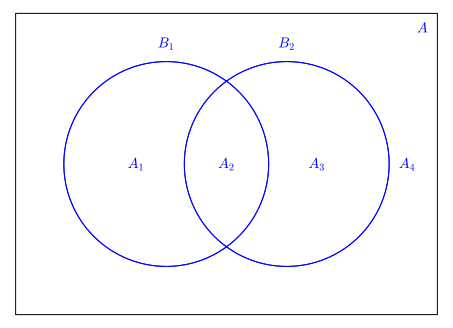
\includegraphics[width=\linewidth]{images/minsets-2.pdf}}%
{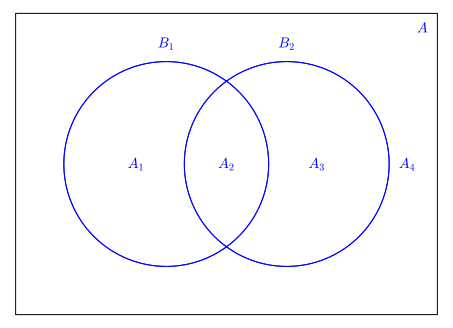
\includegraphics[width=\linewidth]{images/minsets-2.png}}
\end{image}%
\tcblower
\end{figureptx}%
\begin{tableptx}{\textbf{Minsets generated by two sets}}{x:table:tab-minsets-2}{}%
\centering
{\tabularfont%
\begin{tabular}{c}
\(A_1=B_1\cap B_2^c\)\tabularnewline[0pt]
\(A_2=B_1\cap B_2\)\tabularnewline[0pt]
\(A_3= B_1^c\cap B_2\)\tabularnewline[0pt]
\(A_4= B_1^c\cap B_2^c\)
\end{tabular}
}%
\end{tableptx}%
Each \(A_i\) is called a minset generated by \(B_1\) and \(B_2\). We note that each minset is formed by taking the intersection of two sets where each may be either \(B_k\) or its complement, \(B_k^c\). Note also, given two sets, there are \(2^{2}=4\) minsets.%
\par
Minsets are occasionally called \emph{minterms}.%
\par
The reader should note that if we apply all possible combinations of the operations intersection, union, and complementation to the sets \(B_1\) and \(B_2\) of \hyperref[x:figure:fig-minsets-2]{Figure~1}, the smallest sets generated will be exactly the minsets, the minimum sets. Hence the derivation of the term minset.%
\par
Next, consider the Venn diagram containing three sets, \(B_1\), \(B_2\), and \(B_3\). Draw it right now and count the regions! What are the minsets generated by \(B_1\), \(B_2\), and \(B_3\)? How many are there? Following the procedures outlined above, we note that the following are three of the \(2^3=8\) minsets. What are the others?%
\begin{tableptx}{\textbf{Three of the minsets generated by \(B_1\), \(B_2\), and \(B_3\)}}{x:table:tab-some-minsets-3}{}%
\centering
{\tabularfont%
\begin{tabular}{c}
\(B_1\cap B_2\cap B_3^c\)\tabularnewline[0pt]
\(B_1\cap B_2^c\cap B_3\)\tabularnewline[0pt]
\(B_1\cap B_2^c\cap B_3^c\)
\end{tabular}
}%
\end{tableptx}%
\begin{definition}{Minset.}{x:definition:def-Minset}%
\index{Minset}%
Let \(\{B_1, B_2,\ldots,B_n\}\) be a set of subsets of  set \(A\). Sets of the form \(D_1\cap D_2\cap
\cdots \cap D_n\), where each \(D_i\) may be either \(B_i\) or \(B_i^c\), is called a minset generated by \(B_1\), \(B_2\),... and  \(B_n\).%
\end{definition}
\begin{example}{A concrete example of some minsets.}{x:example:ex-minset-example}%
Consider the following concrete example. Let \(A = \{1, 2, 3, 4, 5, 6\}\) with subsets \(B_1 = \{1,3,5\}\) and \(B_2= \{1,2,3\}\). How can we use set operations applied to and produce a partition of \(A\)? As a first attempt, we might try these three sets:%
\begin{tableptx}{\textbf{}}{x:table:tab-subsets-generated-1}{}%
\centering
{\tabularfont%
\begin{tabular}{c}
\(B_1\cap B_2=\{1,3\}\)\tabularnewline[0pt]
\(B_1^c=\{2,4,6\}\)\tabularnewline[0pt]
\(B_2^c=\{4,5,6\}\).
\end{tabular}
}%
\end{tableptx}%
We have produced all elements of \(A\) but we have 4 and 6 repeated in two sets. In place of \(B_1^c\) and \(B_2^c\), let's try \(B_1^c\cap B_2\) and \(B_1\cap B_2^c\), respectively:%
\begin{tableptx}{\textbf{}}{x:table:tab-subsets-generated-2}{}%
\centering
{\tabularfont%
\begin{tabular}{c}
\(B_1^c\cap B_2=\{2\}\) and\tabularnewline[0pt]
\(B_1\cap B_2^c=\{5\}\).
\end{tabular}
}%
\end{tableptx}%
We have now produced the elements 1, 2, 3, and 5 using \(B_1\cap B_2\),  \(B_1^c\cap B_2\) and \(B_1\cap B_2^c\) yet we have not listed the elements 4 and 6. Most ways that we could combine \(B_1\) and \(B_2\) such as \(B_1\cup B_2\) or \(B_1\cup B_2^c\) will produce duplications of listed elements and will not produce both 4 and 6. However we note that \(B_1^c\cap B_2^c= \{4, 6\}\), exactly the elements we need.%
\par
After more experimenting, we might reach a conclusion that each element of \(A\) appears exactly once in one of the four minsets \(B_1\cap B_2\) ,  \(B_1^c\cap B_2\), \(B_1\cap B_2^c\) and \(B_1^c\cap B_2^c\). Hence, we have a partition of \(A\). In fact this is the finest partition of \(A\) in that all other partitions we could generate consist of selected unions of these minsets.%
\par
At this point, we might ask and be able to answer the question ``How many different subsets of our universe can we generate from  \(B_1\) and \(B_2\)?''  The answer is \(2^{\textrm{number of nonempty minsets}}\), which is \(2^4=16\) in this case.  Notice that in general, it would be impossible to find two sets from which we could generate all subsets of \(A=\{1, 2, 3, 4, 5, 6\}\) since there will never be more than four nonempty minsets.   If we allowed ourselves three subsets and tried to generat all sets from them, then the number of minsets would be \(2^3 =8\).  With only six elements in \(A\), there could be six minsets, each containing a single element.  In that case we could generate the whole power set of \(A\).%
\end{example}
\end{subsectionptx}
%
%
\typeout{************************************************}
\typeout{Subsection 1.3.2 Properties of Minsets}
\typeout{************************************************}
%
\begin{subsectionptx}{Properties of Minsets}{}{Properties of Minsets}{}{}{g:subsection:idm352001006720}
\begin{theorem}{Minset Partition Theorem.}{}{x:theorem:th-minset-partition}%
Let \(A\) be a set and let \(B_1\), \(B_2\) \(\ldots\)  , \(B_n\) be subsets of \(A\). The set of nonempty minsets generated by  \(B_1\), \(B_2\) \(\ldots\)  , \(B_n\) is a partition of \(A\).%
\end{theorem}
\begin{proof}{}{g:proof:idm352000951504}
The proof of this theorem is left to the reader.%
\end{proof}
One of the most significant facts about minsets is that any subset of \(A\) that can be obtained from  \(B_1\), \(B_2\) \(\ldots\), \(B_n\), using the standard set operations can be obtained in a standard form by taking the union of selected minsets.%
\begin{definition}{Minset Normal Form.}{x:definition:def-minset-normal-form}%
\index{Minset Normal Form}%
A set is said to be in minset normal form when it is expressed as the union of zero or more distinct nonempty minsets.%
\end{definition}
Notes:%
\par
%
\begin{itemize}[label=\textbullet]
\item{}The union of zero sets is the empty set, \(\emptyset\).%
\item{}Minset normal form is also called \terminology{canonical form}.%
\end{itemize}
%
\begin{example}{Another Concrete Example of Minsets.}{x:example:ex-concrete-minsets-2}%
Let \(U = \{-2,-1,0,1,2\}\), \(B_1= \{0,1,2\}\), and \(B_2= \{0,2\}\).  Then%
\begin{tableptx}{\textbf{}}{g:table:idm352000937536}{}%
\centering
{\tabularfont%
\begin{tabular}{c}
\(B_1\cap B_2=\{0,2\}\)\tabularnewline[0pt]
\(B_1^c\cap B_2 = \emptyset\)\tabularnewline[0pt]
\(B_1\cap B_2^c = \{1\}\)\tabularnewline[0pt]
\(B_1^c\cap B_2^c = \{-2,-1\}\)
\end{tabular}
}%
\end{tableptx}%
In this case, there are only three nonempty minsets, producing the partition \(\{\{0,2\},\{1\},\{-2,-1\}\}\). An example of a set that could not be produced from just \(B_1\) and \(B_2\) is the set of even elements of \(U\), \(\{-2,0,2\}\). This is because \(-2\) and \(-1\) cannot be separated. They are in the same minset and any union of minsets either includes or excludes them both.  In general, there are \(2^3= 8\) different minset normal forms because there are three nonempty minsets. This means that only 8 of the \(2^5=32\) subsets of \(U\) could be generated from  any two sets \(B_1\) and \(B_2\).%
\end{example}
\end{subsectionptx}
%
%
\typeout{************************************************}
\typeout{Exercises 1.3.3 Exercises}
\typeout{************************************************}
%
\begin{exercises-subsection}{Exercises}{}{Exercises}{}{}{x:exercises:exercises-4-3}
\begin{divisionexercise}{1}{}{}{g:exercise:idm352000927904}%
Consider the subsets \(A = \{1, 7, 8\}\), \(B = \{1, 6, 9, 10\}\), and \(C = \{1, 9, 10\}\), where \(U = \{1,2, . . . , 10\}\).%
\par
%
\begin{enumerate}[label=(\alph*)]
\item{}List the nonempty minsets generated by \(A, B, \textrm{ and } C\).%
\item{}How many elements of the power set of \(U\) can be generated by \(A\), \(B\), and \(C\)? Compare this number with \(\mid\mathcal{P}(U)\mid\).  Give an example of one subset that cannot be generated by \(A\), \(B\), and \(C\).%
\end{enumerate}
%
\par\smallskip%
\noindent\textbf{\blocktitlefont Answer}.\hypertarget{g:answer:idm352000927536}{}\quad{}%
\begin{enumerate}[label=(\alph*)]
\item{}\(\displaystyle \{1\}, \{2, 3, 4, 5\}, \{6\}, \{7, 8\}, \{9, 10\}\)%
\item{}\(2^5\) , as compared with \(2^{10}\).   \(\{1, 2\}\) is one of the 992 sets that can't be generated.%
\end{enumerate}
%
\end{divisionexercise}%
\begin{divisionexercise}{2}{}{}{g:exercise:idm352000916368}%
%
\begin{enumerate}[label=(\alph*)]
\item{}Partition \(\{1, 2, .... 9\}\) into the minsets generated by \(B_1= \{5, 6,7\}\), \(B_2 = \{2, 4, 5, 9\}\), and \(B_3 = \{3, 4, 5, 6, 8, 9\}\).%
\item{}How many different subsets of \(\{1, 2, . . . ,9\}\) can you create using \(B_1, B_2\), and \(B_3\) with the standard set operations?%
\item{}Do there exist subsets \(C_1, C_2, C_3\) whose minsets will generate every subset of \(\{1,2, . . . ,9\}\)?%
\end{enumerate}
%
\end{divisionexercise}%
\begin{divisionexercise}{3}{}{}{g:exercise:idm352000927776}%
Partition the set of strings of 0's and 1's of length two or less, using the minsets generated by \(B_1=\{s \mid s \textrm{ has length } 2\}\), and \(B_2= \{s \mid s \textrm{ starts with a }   0\}\).%
\par\smallskip%
\noindent\textbf{\blocktitlefont Answer}.\hypertarget{g:answer:idm352000908720}{}\quad{}\(B_1= \{00, 01, 10, 11\}\) and \(B_2 = \{0, 00, 01\}\) generate minsets \(\{00, 01\}, \{0\}, \{10, 11\}\), and \(\{\lambda , 1\}\). Note: \(\lambda\) is the null string, which has length zero.%
\end{divisionexercise}%
\begin{divisionexercise}{4}{}{}{x:exercise:exercise-minsets-3}%
Let \(B_1, B_2\), and \(B_3\) be subsets of a universal set \(U\),%
\par
%
\begin{enumerate}[label=(\alph*)]
\item{}Symbolically list all minsets generated by \(B_1, B_2\), and \(B_3\).%
\item{}Illustrate with a Venn diagram all minsets obtained in part (a).%
\item{}Express the following sets in minset normal form: \(B_1^c\), \(B_1\cap B_2\) , \(B_1\cup B_2^c\).%
\end{enumerate}
%
\end{divisionexercise}%
\begin{divisionexercise}{5}{}{}{g:exercise:idm352000899504}%
%
\begin{enumerate}[label=(\alph*)]
\item{}Partition \(A = \{0, 1, 2, 3, 4, 5\}\) with the minsets generated by \(B_1= \{0, 2, 4\}\text{  }\)and \(B_2= \{1, 5\}\).%
\item{}How many different subsets of \(A\) can you generate from  \(B_1 \textrm{ and } B_2\)?%
\end{enumerate}
%
\par\smallskip%
\noindent\textbf{\blocktitlefont Answer}.\hypertarget{g:answer:idm352000895616}{}\quad{}%
\begin{enumerate}[label=(\alph*)]
\item{}\(B_1\cap B_2=\emptyset\),  \(B_1\cap B_2^c=\{0,2,4\}\), \(B_1^c\cap B_2=\{1,5\}\), \(B_1^c\cap B_2^c=\{3\}\)%
\item{}\(2^3\), since there are 3 nonempty minsets.%
\end{enumerate}
%
\end{divisionexercise}%
\begin{divisionexercise}{6}{}{}{g:exercise:idm352000892128}%
If \(\left\{B_1, B_2, \ldots , B_n\right\}\) is a partition of \(A\), how many minsets are generated by \(B_1, B_2, \ldots , B_n\)?%
\end{divisionexercise}%
\begin{divisionexercise}{7}{}{}{g:exercise:idm352000890240}%
Prove \hyperref[x:theorem:th-minset-partition]{Theorem~{\xreffont\ref{x:theorem:th-minset-partition}}}%
\par\smallskip%
\noindent\textbf{\blocktitlefont Answer}.\hypertarget{g:answer:idm352000889040}{}\quad{}Let \(a\in A\). For each \(i\), \(a\in B_i\), or \(a\in B_i{}^c\), since \(B_i\cup B_i{}^c=A\) by the complement law. Let \(D_i=B_i\) if \(a\in B_i\), and \(D_i=B_i{}^c\) otherwise. Since \(a\) is in each \(D_i\), it must be in the minset \(D_1\cap  D_2 \cdots \cap D_n\). Now consider two different minsets \(M_1= D_1\cap D_2\cdots \cap D_n\), and \(M_2=G_1\cap G_2\cdots \cap G_n\), where each \(D_i\) and \(G_i\) is either \(B_i\) or \(B_i{}^c\). Since these minsets are not equal, \(D_i\neq G_i\), for some \(i\). Therefore, \(M_1\cap M_2=D_1\cap  D_2 \cdots \cap D_n\cap G_1\cap G_2\cdots \cap G_n=\emptyset\), since two of the sets in the intersection are disjoint. Since every element of \(A\) is in a minset and the minsets are disjoint, the nonempty minsets must form a partition of \(A\). \(\square\)%
\end{divisionexercise}%
\begin{divisionexercise}{8}{}{}{g:exercise:idm352000888288}%
Let \(S\) be a finite set of \(n\) elements. Let \(B_i\), \(i = 1, 2, \ldots , k\) be nonempty subsets of \(S\). There are \(2^{2^k}\) minset normal forms generated by the \(k\) subsets. The number of subsets of \(S\) is \(2^n\). Since we can make \(2^{2^k} > 2^n\) by choosing \(k \geq  \log _2 n\), it is clear that two distinct minset normal-form expressions do not always equal distinct subsets of \(S\). Even for \(k < \log _2 n\), it may happen that two distinct minset normal-form expressions equal the same subset of \(S\). Determine necessary and sufficient conditions for distinct normal-form expressions to equal distinct subsets of \(S\).%
\end{divisionexercise}%
\end{exercises-subsection}
\end{sectionptx}
%
%
\typeout{************************************************}
\typeout{Section 1.4 The Duality Principle}
\typeout{************************************************}
%
\begin{sectionptx}{The Duality Principle}{}{The Duality Principle}{}{}{x:section:s-duality-principle}
%
%
\typeout{************************************************}
\typeout{Subsection 1.4.1 }
\typeout{************************************************}
%
\begin{subsectionptx}{}{}{}{}{}{g:subsection:idm352000870608}
In Section 4.2, we observed that each of the \hyperref[x:table:table-set-laws]{Table~{\xreffont\ref{x:table:table-set-laws}}} labeled 1 through 9 had an analogue \(1^{\prime}\) through \(9^{\prime}\). We notice that each of the laws in one column can be obtained from the corresponding law in the other column by replacing \(\cup\) by \(\cap \), \(\cap \) by \(\cup \), \(\emptyset \) by \(U\), \(U\) by \(\emptyset\), and leaving the complement unchanged.%
\begin{definition}{Duality Principle for Sets.}{x:definition:def-duality-sets}%
Let \(S\) be any identity involving sets and the operations complement, intersection and union. If \(S*\) is obtained from \(S\) by making the substitutions \(\cup  \to  \cap\), \(\cap \to \cup\), \(\emptyset \to U\) , and \(U\to \emptyset\), then the statement \(S*\) is also true and it is called the dual of the statement \(S\).%
\end{definition}
\begin{example}{Example of a dual.}{x:example:ex-dual-example}%
The dual of \((A \cap  B) \cup  \left(A \cap B^c \right) = A\) is \((A\cup B)\cap \left(A\cup B^c\right)=A\).%
\end{example}
One should not underestimate the importance of this concept. It gives us a whole second set of identities, theorems, and concepts. For example, we can consider the dual of \emph{minsets} and \emph{minset normal form} to obtain what is called \emph{maxsets} and \emph{maxset normal form}.%
\end{subsectionptx}
%
%
\typeout{************************************************}
\typeout{Exercises 1.4.2 Exercises}
\typeout{************************************************}
%
\begin{exercises-subsection}{Exercises}{}{Exercises}{}{}{x:exercises:exer-4-4}
\begin{divisionexercise}{1}{}{}{g:exercise:idm352000855408}%
State the dual of each of the following:%
\begin{enumerate}[label=(\alph*)]
\item{}\(A \cup  (B \cap  A) = A\).%
\item{}\(\displaystyle A \cup  \left(\left(B^c \cup  A\right) \cap B\right)^c = U\)%
\item{}\(\displaystyle \left(A \cup  B^c\right)^c \cap  B =A^c\cap B\)%
\end{enumerate}
%
\par\smallskip%
\noindent\textbf{\blocktitlefont Answer}.\hypertarget{g:answer:idm352000851680}{}\quad{}%
\begin{enumerate}[label=(\alph*)]
\item{}\(\displaystyle A\cap (B\cup A)=A\)%
\item{}\(\displaystyle A \cap \left(\left(B^c\cap A\right)\cup B\right)^c=\emptyset\)%
\item{}\(\displaystyle \left(A\cap B^c\right)^c\cup B=A^c\cup B\)%
\end{enumerate}
%
\end{divisionexercise}%
\begin{divisionexercise}{2}{}{}{g:exercise:idm352000855280}%
Examine \mono{[cross-reference to target(s) \textquotedbl{}table-equivalences\textquotedbl{} missing]} and then write a description of the principle of duality for logic.%
\end{divisionexercise}%
\begin{divisionexercise}{3}{}{}{g:exercise:idm352000848256}%
Write the dual of each of the following:%
\begin{enumerate}[label=(\alph*)]
\item{}\(\displaystyle p\lor \neg ((\neg q\lor p)\land q)\Leftrightarrow 1\)%
\item{}\((\neg (p \land  (\neg  q ))) \lor  q\Leftrightarrow (\neg p \lor  q)\).%
\end{enumerate}
%
\par\smallskip%
\noindent\textbf{\blocktitlefont Answer}.\hypertarget{g:answer:idm352001266480}{}\quad{}%
\begin{enumerate}[label=(\alph*)]
\item{}\(\displaystyle (p \land \neg (\neg  q \land p)\lor q) \Leftrightarrow 0\)%
\item{}\(\displaystyle (\neg (p \lor  (\neg q)))\land q \Leftrightarrow ((\neg p) \land q)\)%
\end{enumerate}
%
\end{divisionexercise}%
\begin{divisionexercise}{4}{}{}{g:exercise:idm352000843104}%
Use the principle of duality and the definition of minset to write the definition of maxset.%
\end{divisionexercise}%
\begin{divisionexercise}{5}{}{}{g:exercise:idm352000842256}%
Let \(A = \{1,2, 3,4, 5, 6\}\) and let \(B_1 = \{1, 3, 5\}\) and \(B _2 = \{1,2, 3\}\).%
\par
%
\begin{enumerate}[label=(\alph*)]
\item{}Find the maxsets generated by \(B_1\) and \(B_2\). Note the set of maxsets does not constitute a partition of \(A\). Can you explain why?%
\item{}Write out the definition of maxset normal form.%
\item{}Repeat \hyperlink{x:exercise:exercise-minsets-3}{Exercise~{\xreffont 1.3.3.4}}  for maxsets.%
\end{enumerate}
%
\par\smallskip%
\noindent\textbf{\blocktitlefont Answer}.\hypertarget{g:answer:idm352000836896}{}\quad{}The maxsets are:%
\par
%
\begin{itemize}[label=\textbullet]
\item{}\(\displaystyle B_1\cup B_2=\{1,2,3,5\}\)%
\item{}\(\displaystyle B_1\cup B_2{}^c=\{1,3,4,5,6\}\)%
\item{}\(\displaystyle B_1{}^c\cup B_2=\{1,2,3,4,6\}\)%
\item{}\(\displaystyle B_1{}^c\cup B_2{}^c=\{2,4,5,6\}\)%
\end{itemize}
%
\par
They do not form a partition of \(A\) since it is not true that the intersection of any two of them is empty. A set is said to be in \terminology{maxset normal form} when it is expressed as the intersection of distinct nonempty maxsets or it is the universal set \(U\).%
\end{divisionexercise}%
\begin{divisionexercise}{6}{}{}{g:exercise:idm352000831488}%
What is the dual of the expression in \hyperlink{x:exercise:ex-generalized_distrib}{Exercise~{\xreffont 1.1.5.5}} ?%
\end{divisionexercise}%
\end{exercises-subsection}
\end{sectionptx}
\end{chapterptx}
%
%% A lineskip in table of contents as transition to appendices, backmatter
\addtocontents{toc}{\vspace{\normalbaselineskip}}
%
%
%
\typeout{************************************************}
\typeout{Appendix A Determinants}
\typeout{************************************************}
%
%
\appendix
%
\begin{appendixptx}{Determinants}{}{Determinants}{}{}{x:appendix:app-determinants}
\begin{introduction}{}%
In Chapter 5 we defined the determinant of a \(2 \times 2\) matrix for the sole purpose of providing some hands-on experience in the computation of inverses of \(2 \times 2\) matrices. In this appendix we will define the determinant of any square matrix, and summarize the main properties of determinants.%
\end{introduction}%
%
%
\typeout{************************************************}
\typeout{Section A.1 Definition}
\typeout{************************************************}
%
\begin{sectionptx}{Definition}{}{Definition}{}{}{g:section:idm352000826528}
Associated with every square matrix is a number called its determinant. The most important information it provides us with is whether the matrix is invertible. A matrix has an inverse if and only if its determinant is nonzero.  If \(A\) is a square matrix, then the determinant of \(A\) is commonly denoted either \(\det(A)\)  or \(\lvert A \rvert\).   Strictly speaking, we only need to define the determinant of a \(1 \times 1\) matrix here and then define the higher ordered ones recursively, but for convenience we also recall the definition of the determinant of a \(2 \times 2\) matrix.%
\begin{definition}{Determinant of \(1 \times 1\) and a \(2 \times 2\) matrices.}{x:definition:def-determinant-basis}%
\index{Determinant!\(1 \times 1\) and a \(2 \times 2\) cases}%
%
\begin{itemize}[label=\textbullet]
\item{}If \(A\) is a \(1 \times 1\) matrix, then \(\lvert A \rvert = A_{1,1}\)%
\item{}If \(A\) is a \(2 \times 2\) matrix, then \(\lvert A \rvert = A_{1,1} A_{2,2} - A_{1,2} A_{2,1}\)%
\end{itemize}
%
\end{definition}
We now proceed to define the determinant of an \(n \times n\) matrix where \(n > 2\). This definition requires two preliminary definitions those of minors and cofactors.%
\begin{definition}{Matrix Minor.}{x:definition:def-minor}%
\index{Minor}%
\label{g:notation:idm352000813200}%
Let \(A\) be an \(n \times n\) matrix, \(n \geq 2\). The determinant of the \((n-1) \times (n-1)\) matrix formed by removing the \(i^{th}\) row and  \(j^{th}\) column of \(A\) is the minor denoted by \(M(A)_{i,j}\).%
\end{definition}
\begin{example}{}{x:example:example-minor-3-by-3}%
Let \(A = \begin{pmatrix}
3 & 4 & 1 \\
1 & 3 & 4 \\
4 & 1 & 3 
\end{pmatrix} \) then \(A\) has nine minors, one of which is%
\begin{equation*}
M(A)_{1,1} = \begin{vmatrix}
3 & 4 \\
1 & 3 
\end{vmatrix} = 3 \cdot 3 - 4 \cdot 1 =5
\end{equation*}
%
\par
For our purposes in computing \(\lvert A \rvert\), we only need minors corresponding to any one row or column.  Completing the minors in the first row we have \(M(A)_{1,2} = -13 \)   and  \(M(A)_{1,3} = -11 \)%
\end{example}
\begin{definition}{Cofactor.}{x:definition:def-cofactor}%
\index{Cofactor}%
\label{g:notation:idm352000803344}%
Let \(A\) be an \(n \times n\) matrix, \(n \geq 2\). The \(i^{th}\) row, \(j^{th}\) column cofactor of  \(A\), denoted \(C(A)_{i,j}\), is defined by%
\begin{equation*}
C(A)_{i,j} = (-1)^{i+j} M(A)_{i,j}
\end{equation*}
%
\end{definition}
\begin{example}{}{x:example:example-cofactors-3-by-3}%
Using the values of minors computed in \hyperref[x:example:example-minor-3-by-3]{Example~3}, we have \(C(A)_{1,1} = (-1)^2 M(A)_{1,1} = 5\), \(C(A)_{1,2} = (-1)^3 M(A)_{1,2} = 13\), and \(C(A)_{1,3} = (-1)^4 M(A)_{1,3} = -11\).%
\end{example}
Finally, we will define the determinant of a square matrix. Our definition is practical in that you can apply it easily to any matrix.  It isn't the most general, nor is it the best definiton for the purposes of proving properties of determinants.  The more general definition is beyond our current scope, but can be easily stated with background in permutation groups.%
\begin{definition}{Determinant of a Square Matrix.}{x:definition:def-determinant-general}%
\index{Determinant}%
\label{g:notation:idm352000793792}%
Let \(A\) be an \(n \times n\) matrix, \(n \geq 2\). The determinant of \(A\) is equal to%
\begin{equation*}
\sum_{j=1}^{n} A_{1,j}\cdot C(A)_{1,j} 
\end{equation*}
%
\end{definition}
Our definition of a determinant involves what is called expansion along the first row of the matrix A. It is certainly not obvious, but it is true, that the determinant of a matrix can be found by expanding along any row or any column.%
\begin{example}{}{x:example:example-determinant-3-3}%
We have computed the cofactors for row 1 of \(A = \begin{pmatrix}
3 & 4 & 1 \\
1 & 3 & 4 \\
4 & 1 & 3 
\end{pmatrix} \) above and so the determinant is only a few operations away.%
\begin{equation*}
\begin{split}
\lvert A \rvert &= A_{1,1}\cdot C(A)_{1,1} +A_{1,2}\cdot C(A)_{1,2}+A_{1,3}\cdot C(A)_{1,3}\\
&= 3\cdot 5 + 4\cdot 13 + 1 \cdot (-11)\\
&= 56
\end{split}
\end{equation*}
%
\end{example}
\begin{example}{}{x:example:characteristic-polynomial}%
\index{Characteristic Polynomial}%
Associated with any square matrix, \(A\), is a characteristic polynomial which is defined to be the \(\lvert A - \lambda I \rvert\).   The roots of this polynomial are the eigenvalues of the matrix. Here, we compute the characteristic polynomial of \(A = \begin{pmatrix}
3 & 4 & 1 \\
1 & 3 & 4 \\
4 & 1 & 3 
\end{pmatrix}\).%
\par
To compute the determinant we expand along the first row.%
\begin{equation*}
\begin{split}
\det{(A - \lambda I)} &=  \begin{vmatrix}
3 - \lambda & 4 & 1 \\
1 & 3 - \lambda & 4 \\
4 & 1 & 3 - \lambda 
\end{vmatrix}\\
&= (3-\lambda)\cdot  \begin{vmatrix}
3 - \lambda & 4 \\
1 & 3 - \lambda 
\end{vmatrix}
+ 4 \cdot (-1)\cdot \begin{vmatrix}
1 & 4 \\
4 &  3 - \lambda
\end{vmatrix}
+ 1\cdot  \begin{vmatrix}					
1 & 3 - \lambda  \\
4 & 1  
\end{vmatrix} \\
&=(3-\lambda)((3-\lambda)^2-4) - 4((3-\lambda)-16) + (1-4(3-\lambda))\\
&=-\lambda ^3+9 \lambda ^2-15 \lambda +56
\end{split}
\end{equation*}
%
\end{example}
\end{sectionptx}
%
%
\typeout{************************************************}
\typeout{Section A.2 Computation}
\typeout{************************************************}
%
\begin{sectionptx}{Computation}{}{Computation}{}{}{g:section:idm352000826400}
Our definition of determinant can be applied to estimate the worst case for the time to evaluate an \(n \times n\) determinant.   Let \(M(n)\) be the number of multiplications to evaluate an \(n \times n\) determinant.  Then we have  \(M(2)=2\).  To determine the value of \(M(3)\) we observe that this requires the computation of three minors, each a two by two matrix, and then a multiplication of each of them by the entries in row 1.  Therefore, \(M(3)= 3 M(2) + 3 = 9\).  Using the same logic in general, we have \(M(n)= n M(n-1) + n\).  The formula can be derived to be \(M(n) =n! \sum _{k=1}^n \frac{1}{k!}\).  For large \(n\) this is approximately \(e\cdot n!\).  Fortunately, there are ways to reduce the number of multiplications using properties of determinants, which we list here without proof.%
\begin{theorem}{Properties of Determinants.}{}{x:theorem:determinant-properties}%
Let \(A\)  and \(B\) be \(n \times n\) matrices, where \(n \geq 2\).%
\begin{enumerate}
\item{}\(\lvert A \rvert\) can be found by expanding along any row or any column.%
\item{}If two rows (or columns) of \(A\) are interchanged, \(\lvert A \rvert\) changes sign.%
\item{}The value of a determinant is unchanged if a multiple of one row (or column) of \(A\) is added to another row (or column) of \(A\) .%
\item{}If one row (or column) of a matrix \(A\) is multiplied by a constant \(c\), then the value of \(\lvert A \rvert\) is multiplied by \(c\).%
\item{}\(\lvert A B \rvert = \lvert A \rvert \cdot \lvert B \rvert\).%
\item{}\(\lvert I \rvert  = 1\) where \(I\) is the \(n \times n\) identity matrix.%
\end{enumerate}
%
\end{theorem}
Based on these properties, here are a few corollaries.%
\begin{corollary}{Further Properties.}{}{x:corollary:determinant-corollaries}%
Let \(A\)  and \(B\) be \(n \times n\) matrices, where \(n \geq 2\).%
\begin{enumerate}
\item{}If a row (or column) of \(A\) consists entirely of zeros, then \(\lvert A \rvert = 0\).%
\item{}If a matrix \(A\) has two equal rows (or columns) then \(\lvert A \rvert = 0\).%
\item{}If any row (or column) of \(A\) is a scalar multiple of any other row (or column) of \(A\), then \(\lvert A \rvert = 0\).%
\item{}\(\lvert A^{-1} \rvert =\frac{1}{\lvert A \rvert}\) , if \(A^{-1}\) exists.%
\end{enumerate}
%
\end{corollary}
\begin{example}{Computatation of a determinant by row reduction.}{x:example:determinant-by-reduction}%
We will apply some of these properties, most notably the first and third of \hyperref[x:theorem:determinant-properties]{Theorem~1}, to compute a four by four determinant without doing as many multiplications as expected.  We will use SageMath to do the calculations for us.  In SageMath, as in Python, numbering starts at zero, so we will describe the process using that numbering system.  Let \(A=\begin{pmatrix}1 & 3 & 4 & 7\\
1 & 3 & 4 & 4\\
6 & 6 & 7 & 8\\
3 & 3 & 7 & 5
\end{pmatrix}\)%
\par
Our strategy will be to create a column that is mostly zero so that we can expand along that column and only need to compute one cofactor.  That will be the 0th column.  To do that we do the following row operations.  We subtract row 0 from row 1, replacing row 1 with that result.  Then we subtract six time row 0 from row 2, producing a new row 2.  Finally, three times row 0 is subtracted from row 3 to produce a new row 3.  The SageMath code below accomplishes this and produces a new matrix, \(B\), which has the same determinant.%
\begin{sageinput}
A=matrix([[1,3,4,7],[2,3,4,4],[5,6,7,4],[3,3,7,5]])
B=matrix([A[0],A[1]-2*A[0],A[2]-5*A[0],A[3]-3*A[0]]);B
\end{sageinput}
\begin{sageoutput}
[  1   3   4   7]
[  0  -3  -4 -10]
[  0  -9 -13 -31]
[  0  -6  -5 -16]
\end{sageoutput}
Expanding this matrix along the column zero, we need only compute a single three by three cofactor.  We will go one step further and do row operations to get a matrix with zeros in rows 2 and 3 of column 1.  The SageMath code below tells what we are doing.%
\begin{sageinput}
C=matrix([B[0],B[1],B[2]-3*B[1],B[3]-2*B[1]]);C
\end{sageinput}
\begin{sageoutput}
[  1   3   4   7]
[  0  -3  -4 -10]
[  0   0  -1  -1]
[  0   0   3   4]
\end{sageoutput}
We are at a point where we can do the final calculation very easily.%
\begin{equation*}
\lvert A \rvert = \lvert C \rvert = 1 \cdot(-3 \cdot (-1\cdot 4 - 3\cdot (-1)))= 3
\end{equation*}
SageMath has a determinant function, \mono{det}, that we can use to verify this calculation:%
\begin{sageinput}
A=matrix([[1,3,4,7],[2,3,4,4],[5,6,7,4],[3,3,7,5]])
det(A)
\end{sageinput}
\begin{sageoutput}
3
\end{sageoutput}
\end{example}
\end{sectionptx}
\end{appendixptx}
%
%
\typeout{************************************************}
\typeout{Appendix B Python and SageMath}
\typeout{************************************************}
%
\begin{appendixptx}{Python and SageMath}{}{Python and SageMath}{}{}{x:appendix:app-pythonsage}
\begin{introduction}{}%
SageMath (originally Sage) is a computer algebra system that is built on top of Python, which is a popular general-purpose programming language.  In this appendix we highlight a few features of Python through a series of SageMath cells.   Pure Python code can generally be evaluated in these cells and most of what you see here is just Python.   There are exceptions. For example, SageMath has  enhanced capabilities to work with sets.  In Python, the expression \mono{set([0,1,2,3])} is a set of four integers, and certain basic set operations can be performed on these types of expressions.  This is a valid expression in SageMath too, but a different SageMath expression, \mono{Set([0,1,2,3])}, with a capital S, has enhanced properties.  For example, we can create the power set of the SageMath expression, which we do in the discussion of iterators.%
\end{introduction}%
%
%
\typeout{************************************************}
\typeout{Section B.1 Python Iterators}
\typeout{************************************************}
%
\begin{sectionptx}{Python Iterators}{}{Python Iterators}{}{}{x:section:app-python-iterators}
\begin{introduction}{}%
All programming languages allow for looping.  A common form of loop is one in which a series of instructions are executed for each value of some index variable, commonly for values between two integers.  Python allows a bit more generality by having structures called ``iterators'' over which looping can be done.   An iterator can be as simple as a list, such as \mono{[0,1,2,3]}, but also can be a power set of a finite set, as we see below, or the keys in a dictionary, which is described in the next section.%
\end{introduction}%
%
%
\typeout{************************************************}
\typeout{Subsection B.1.1 Counting Subsets}
\typeout{************************************************}
%
\begin{subsectionptx}{Counting Subsets}{}{Counting Subsets}{}{}{g:subsection:idm352000744560}
Suppose we want to count the number of subsets of \(\{0,1,2,...,9\}\) that contain no adjacent elements.  First, we will define our universe and its power set.  The plan will be to define a function that determines whether a subset is "valid" in the sense that it contains no adjacent elements.  Then we will iterate over the subsets, counting the valid ones.  We know that the number of all subsets will be 2 raised to the number of elements in \(U\), which would be \(2^{10}=1024\), but let's check.%
\begin{sageinput}
U=Set(range(10))
power_set=U.subsets()
len(power_set)
\end{sageinput}
\begin{sageoutput}
1024
\end{sageoutput}
The validity check in this case is very simple.  For each element, \(k\), of a set, \(B\), we ask whether its successor, \(k+1\), is also in the set.  If we never get an answer of "True" then we consider the set valid.  This function could be edited to define validity in other ways to answer different counting questions.  It's always a good idea to test your functions, so we try two tests, one with a valid set and one with an invalid one.%
\begin{sageinput}
def valid(B):
    v=true
    for k in B:
        if k+1 in B:
            v=false
            break
    return v
[valid(Set([1,3,5,9])),valid(Set([1,2,4,9]))]
\end{sageinput}
\begin{sageoutput}
[True, False]
\end{sageoutput}
Finally we do the counting over our power set, incrementing the count variable with each valid set.%
\begin{sageinput}
count=0
for B in power_set:
    if valid(B):
        count+=1
count
\end{sageinput}
\begin{sageoutput}
144
\end{sageoutput}
\end{subsectionptx}
\end{sectionptx}
%
%
\typeout{************************************************}
\typeout{Section B.2 Dictionaries}
\typeout{************************************************}
%
\begin{sectionptx}{Dictionaries}{}{Dictionaries}{}{}{x:section:app-pythonsage-dictionaries}
%
%
\typeout{************************************************}
\typeout{Subsection B.2.1 Colors of Fruits}
\typeout{************************************************}
%
\begin{subsectionptx}{Colors of Fruits}{}{Colors of Fruits}{}{}{g:subsection:idm352000736976}
In Python and SageMath, a dictionary is a convenient data structure for establishing a relationship between sets of data.  From the point of view of this text, we can think of a dictionary as a concrete realization of a relation between two sets or on a single set.  A dictionary resembles a function in that there is a set of data values called the \mono{keys}, and for each key, there is a \mono{value}.  The value associated with a key can be almost anything, but it is most commonly a list.%
\par
To illustrate the use of dictionaries, we will define a relationship between colors and fruits.  The keys will be a set of colors and values associated with each color will be a list of fruits that can take on that color. We will demonstrate how to initialize the dictionary and how to add to it.  The following series of assignments have no output, so we add a print statement to verify that this cell is completely evaluated.%
\begin{sageinput}
fruit_color={}
fruit_color['Red']=['apple','pomegranate','blood orange']
fruit_color['Yellow']=['banana','apple','lemon']
fruit_color['Green']=['apple','pear','grape','lime']
fruit_color['Purple']=['plum','grape']
fruit_color['Orange']=['orange','pineapple']
print('done')
\end{sageinput}
\begin{sageoutput}
done
\end{sageoutput}
We distinguish a color from a fruit by capitalizing colors but not fruit.  The keys of this dictionary are the colors.  The \mono{keys()} method returns an interator; so to get a list of keys we wrap the result with \mono{list()}.%
\begin{sageinput}
list(fruit_color.keys())
\end{sageinput}
\begin{sageoutput}
['Purple', 'Orange', 'Green', 'Yellow', 'Red']
\end{sageoutput}
As an afterthought, we might add the information that a raspberry is red as follows. You have to be careful in that if 'Red' isn't already in the dictionary, it doesn't have a value. This is why we need an if statement.%
\begin{sageinput}
if 'Red' in fruit_color:
    fruit_color['Red']=fruit_color['Red']+['raspberry']
else:
    fruit_color['Red']=['raspberry']
fruit_color['Red']
\end{sageinput}
\begin{sageoutput}
['apple', 'pomegranate', 'blood orange', 'raspberry']
\end{sageoutput}
A dictionary is iterable, with an iterator taking on values that are the keys.  Here we iterate over our dictionary to output lists consisting of a color followed by a list of fruits that come in that color.%
\begin{sageinput}
for fruit in fruit_color:
    print([fruit,fruit_color[fruit]])
\end{sageinput}
\begin{sageoutput}
['Purple', ['plum', 'grape']]
['Orange', ['orange', 'pineapple']]
['Green', ['apple', 'pear', 'grape', 'lime']]
['Yellow', ['banana', 'apple', 'lemon']]
['Red', ['apple', 'pomegranate', 'blood orange','raspberry']]
\end{sageoutput}
We can view a graph of this relation between colors and fruits, but the default view is a bit unconventional.%
\begin{sageinput}
DiGraph(fruit_color).plot()
\end{sageinput}
\begin{sageoutput}

\end{sageoutput}
With a some additional coding we can line up the colors and fruits in their own column. First we set the positions of colors on the left with all \(x\)-coordinates equal to -5 using another dictionary called \mono{vertex\_pos}.%
\begin{sageinput}
vertex_pos={}
k=0
for c in fruit_color.keys():
    vertex_pos[c]=(-5,k)
    k+=1
vertex_pos
\end{sageinput}
\begin{sageoutput}
{'Purple': (-5, 0), 'Orange': (-5, 1), 'Green': (-5, 2), 'Red': (-5, 4), 'Yellow': (-5, 3)}
\end{sageoutput}
Next, we place the fruit vertices in another column with \(x\)-coordinates all equal to 5. In order to do this, we first collect all the fruit values into one set we call \mono{fruits}.%
\begin{sageinput}
fruits=Set([ ])
for v in fruit_color.values():
     fruits=fruits.union(Set(v))
k=0
for f in fruits:
    vertex_pos[f]=(5,k)
    k+=1
vertex_pos
\end{sageinput}
\begin{sageoutput}
{'blood orange': (5, 0), 'grape': (5, 1), 'apple': (5, 2), 'Purple': (-5, 0), 'plum': (5, 10), 'pomegranate': (5, 3), 'pear': (5, 4), 'Yellow': (-5, 3), 'orange': (5, 7), 'Green': (-5, 2), 'pineapple': (5, 6), 'Orange': (-5, 1), 'lemon': (5, 8), 'raspberry': (5, 9), 'banana': (5, 5), 'Red': (-5, 4), 'lime': (5, 11)}
\end{sageoutput}
Now the graph looks like a conventional graph for a relation between two different sets.  Notice that it's not a function.%
\begin{sageinput}
DiGraph(fruit_color).plot(pos=vertex_pos,vertex_size=1)
\end{sageinput}
\begin{sageoutput}
Graphics object consisting of 33 graphics primitives
\end{sageoutput}
\end{subsectionptx}
\end{sectionptx}
\end{appendixptx}
%
\backmatter
%
%
%
\typeout{************************************************}
\typeout{References  References}
\typeout{************************************************}
%
\begin{references-chapter-numberless}{References}{}{References}{}{}{g:references:idm352000736848}
%% If this is a top-level references
%%   you can replace with "thebibliography" environment
\begin{referencelist}
\bibitem[1]{x:biblio:biblio-allenby-1983}\hypertarget{x:biblio:biblio-allenby-1983}{}Allenby, R.B.J.T, \textit{Rings, Fields and Groups}, Edward Arnold, 1983.
\bibitem[2]{x:biblio:biblio-appel-1976}\hypertarget{x:biblio:biblio-appel-1976}{}Appel, K., and W. Haken, \textit{Every Planar Map Is 4-colorable},  Bull, Am. Math. Soc. 82 (1976): 711-12.
\end{referencelist}
\end{references-chapter-numberless}
%
%% The index is here, setup is all in preamble
%% Index locators are cross-references, so same font here
{\xreffont\printindex}
%
\end{document}